\chapter{Conservative Model Order Reduction of Fluid Flow} \label{chapter:7}

In \Cref{chapter:4,chapter:5,chapter:6} it is discussed how MOR can be modified to ensure conservation of symmetries and invariants in the context of Hamiltonian system. A reduced Hamiltonian, as an approximation of the Hamiltonian for the original system, is introduced for the reduced system. Conservation of a skew-symmetric form can then ensure correct evolution of the reduced system and conservation of the reduced Hamiltonian. In this chapter, we apply the same principle to construct a MOR technique for the fluid flow that conserves energy of the flow.

Large scale simulations of fluid flows arise in a wide range of disciplines and industries. Therefore, MOR of fluid flows, specially when advective terms are dominant, is important. It is well known that conservation of the energy, specially kinetic energy, is essential for a qualitatively correct numerical integration of fluid flows. Conventional model reduction techniques often violate conservation of mass, momentum \cite{carlberg2018conservative}, or energy in fluid flows which result in an unstable reduced system, in particular for long time-integration. \edit{In \cite{barone2009stable} an entropy stable model reduction method for linear compressible flows is presented by considering an entropy-stable formulation of linearized compressible flows. Furthermore, a conservative model reduction for finite-volume models is presented in \cite{carlberg2018conservative} that that conserves any quantity conserved by the finite-volume scheme. This method finds a reduced linear subspace that ensures conservation of quantities by solving an optimization problem with, generally nonlinear, equality constraints.}

Skew-symmetric formulation of fluid flows constructs a skew-symmetric differential operator, acting on the momentum vector field, that ensures conservation of quadratic invariants, such as energy. Combined with centered time and space discretization schemes, typically a finite differences discretization method, they recover time-symmetries of a fluid at the discrete level. Such discretization schemes are studies comprehensively over the past few decades and can be found in the works of \cite{morinishi2010skew,morinishi1998fully,desjardins2008high,tadmor1984skew,reiss2014conservative} and the references therein.

This chapter discusses how to preserve skew-symmetry of the differential operators at the level of the reduced system. This results in conservation of quadratic invariants. \edit{The conservation of quantities in the proposed method is guaranteed through the mathematical formulation of the reduced system, for any orthonormal reduced basis. Therefore, the offline computational costs of this method is comparable with conventional MOR techniques. However, other conservative model reduction methods, e.g. \cite{carlberg2018conservative}, often require solving multiple nonlinear optimization problems to ensure conservation. This can significantly increase the offline computational cost.} Furthermore, we show that the reduced system, as a system of coupled differential equations, contains quadratic invariants and an associated energy which approximates the energy of the high-fidelity system. Therefore, a proper time stepping scheme preserves the reduced representation of the energy, and therefore, the loss in energy due to model reduction remains constant in time.Furthermore, we demonstrate, through numerical experiments, that a quasi-skew-symmetric form of fluid flow, i.e. a formulation where only spacial differential operators are in a skew-symmetric form, offer remarkable stability properties in terms of MOR. This allows an explicit time-integration to be utilized while recovering robustness of skew-symmetric forms at the reduced level.

The rest of this chapter is organized as follows. We discuss skew-symmetric and conservatives methods for compressible and incompressible fluid flows in \Cref{p4.sec:skew}. Conservative and energy-preserving model reduction of fluid flows is discussed in \Cref{p4.sec:mor_skew}. We evaluate the performance of the method through numerical simulations of incompressible and compressible fluid flow in \Cref{p4.sec:res}. We also apply the method to construct a reduced system for the continuous variable resonance combustor, a one dimensional reaction-diffusion model for a rocket engine. Finally, we present conclusive remarks in \Cref{p4.sec:con}.

\edit{The main contribution of this chapter is the introduction of a conservative model reduction technique for compressible and incompressible fluids in skew-symmetric form. 
}

\section{Skew Symmetric and Centered Schemes for Fluid Flows} \label{p4.sec:skew}

In this section we summarize the conservation properties of skew-symmetric forms and discretization schemes, following, closely, the works of \cite{morinishi2010skew,morinishi1998fully,tadmor1984skew,reiss2014conservative}.

\subsection{Conservation Laws} \label{p4.sec:skew.1}
In the context of fluid flows, transport of conserved quantities, can be expressed as
\begin{equation} \label{p4.eq:3.1}
	\frac{\partial }{\partial t} \rho \varphi + \nabla \cdot ( \rho u \varphi  ) = \nabla \cdot F_{\varphi}\quad \text{defined in} \quad \Omega \subset \mathbb R^{d}.
\end{equation}
Here, $d = 1,2$ or $3$, $\rho:\Omega\to \mathbb R$ is the density, $u: \Omega \to \mathbb R^{d}$ is the velocity vector field, $\varphi$ is a measured scalar quantity of the flow, and $F_{\varphi}$ is the flux function associated to $\varphi$. Integration of \eqref{p4.eq:3.1} over $ \Omega$ yields
\begin{equation} \label{p4.eq:3.2}
	\frac{d}{dt} \int_{\Omega} \rho \varphi \ dx = \int_{\partial \Omega} (F_{\varphi} - \rho u \varphi) \cdot \hat n\ ds,
\end{equation}
where $\partial \Omega$ is the boundary of $\Omega$, and $\hat n$ is the unit outward normal vector to $\partial \Omega$. \edit{This means that the quantity $(\rho\varphi)$ is explicitly conserved over control volumes}. Therefore, \eqref{p4.eq:3.2} is referred to as the \emph{conservative form} and the convective term in \eqref{p4.eq:3.1} is referred to as the \emph{divergence form}. However, using the \emph{continuity equation}
\begin{equation} \label{p4.eq:3.3}
	\frac{\partial }{\partial t} \rho + \nabla \cdot (\rho u) = 0,
\end{equation}
we can rewrite \eqref{p4.eq:3.1} as
\begin{equation} \label{p4.eq:3.4}
	\rho \frac{\partial }{\partial t} \varphi + (\rho u)\cdot \nabla \varphi = \nabla \cdot F_{\varphi}.
\end{equation}
The convective term in this formulation is referred to as the \emph{advective form}. The \emph{skew-symmetric} form of the convective term is obtained by the arithmetic average of the divergent and the advective form:
\begin{equation} \label{p4.eq:3.5}
	\frac{1}{2} \left( \rho \frac{\partial }{\partial t} \varphi + \frac{\partial }{\partial t} (\rho \varphi) \right) + \frac 1 2 \left( (\rho u)\cdot \nabla \varphi + \nabla \cdot (\rho u \varphi) \right) = \nabla \cdot F_{\varphi}.
\end{equation}
Multiplying \eqref{p4.eq:3.5} with $\varphi$ yields
\edit{
\begin{equation}
	\frac{1}{2} \left( \rho \varphi \frac{\partial }{\partial t} \varphi + \varphi \frac{\partial }{\partial t} (\rho \varphi) \right) + \frac 1 2 \left( (\rho u \varphi)\cdot \nabla \varphi + \varphi \nabla \cdot (\rho u \varphi) \right) = \varphi \nabla \cdot F_{\varphi}.
\end{equation}
Using the product rule, we recover
}
\begin{equation}
	\frac{\partial }{\partial t} \rho \varphi^2 + \nabla \cdot ( \rho u \varphi^2  ) = \varphi \nabla \cdot F_{\varphi}.
\end{equation}
Therefore, $\rho \varphi^2$ is a conserved quantity for a flux-free $\varphi$. Since the divergence, the advective and the skew-symmetric forms are identical at the continuous level, $\varphi^2$ is a conserved quantity for all forms. However, the equivalence of these forms is not preserved through a general discretization scheme and we can not expect $\varphi^2$ to be a conserved quantity at the discrete level. To motivate numerical advantages of the skew-symmetric form consider the operator 
\begin{equation}
	S_{\rho u}(\cdot) = \frac 1 2 ( [ \nabla \cdot \rho u ](\cdot) + (\rho u)\cdot \nabla(\cdot) ),
\end{equation}
\edit{where $[ \nabla \cdot \rho u ](x) = \nabla \cdot( \rho u x) $}. With a proper set of boundary condition, this operator is a skew-adjoint operator on $L^2$. Here, $[\cdot]$ indicates that the inside of the brackets act as a differential operator. This skew-adjoint property is used later to show the conservation of some quadratic quantities in \eqref{p4.eq:3.1}. Similarly, we can define a skew-adjoint operator with respect to the time variable as
\begin{equation}
	S_{\rho,\partial_t} = \frac{1}{2} \left( \rho \frac{\partial}{\partial t} + [ \frac{\partial}{\partial t} \rho] \right).
\end{equation}
Here, the subscript $\partial_t$ is to emphasize that $S_{\rho,\partial_t}$ is a differential operator with respect to $t$. A proper time and space discretization of $S_{\rho u}$ and $S_{\rho,\partial_t}$ can preserve the skewness property.

Numerical time integration of \eqref{p4.eq:3.5} can be challenging since the time differentiation of different variables is present. Following \cite{morinishi2010skew}, we have
\edit{
\begin{equation}
\begin{aligned}
	\frac{1}{2}\left( \frac{\partial}{\partial t}(\rho \varphi) + \rho \frac{\partial}{\partial t} \varphi \right) = \left( \frac{\partial}{\partial t}(\rho \varphi) - \frac{\varphi}{2} \frac{\partial}{\partial t} \rho \right) &= \left( \rho \frac{\partial}{\partial t} \varphi + \frac{\varphi}{2} \frac{\partial}{\partial t} \rho \right) \\
	&= \sqrt{\rho } \frac{\partial }{\partial t} (\sqrt \rho \varphi ),
\end{aligned}
\end{equation}
where the product rule is used in the last step.} Substituting this into \eqref{p4.eq:3.5} yields
\begin{equation} \label{p4.eq:3.6}
	\sqrt{\rho } \frac{\partial }{\partial t} (\sqrt \rho \varphi ) + S_{\rho u}(\varphi) = \nabla \cdot F_{\varphi}.
\end{equation}
Time integration of this form is presented in \cite{morinishi2010skew,reiss2014conservative}. Note that one can also generate a quasi-skew-symmetric form \cite{blaisdell1991numerical,morinishi2003dns} of \eqref{p4.eq:3.1} as
\begin{equation} \label{p4.eq:3.7}
	\frac{\partial }{\partial t} (\rho \varphi) + \edit{ \frac 1 2 \left( \nabla \cdot(\rho u \varphi) + \rho u \cdot \nabla \varphi + \varphi \nabla \cdot(\rho u) \right) } = \nabla \cdot F_{\varphi}.
\end{equation}
\edit{
Here, we substitute the convective term in \eqref{p4.eq:3.1} with
\begin{equation}
	\nabla \cdot(\rho u \varphi) = \frac 1 2 (2\nabla \cdot(\rho u \varphi)) = \frac 1 2 \left( \nabla \cdot(\rho u \varphi) + \rho u \cdot \nabla \varphi + \varphi \nabla \cdot(\rho u) \right).
\end{equation}
}
Even though this is not a fully skew-symmetric form (skew-symmetric only in space), the numerical stability of this form is significantly better than the divergence and advective form \cite{morinishi2010skew,blaisdell1991numerical,morinishi2003dns}. Note that this quasi-skew-symmetric form is identical to the skew-symmetric form in the incompressible limit.

\subsection{Incompressible Fluid} \label{p4.sec:skew.2}
Consider the governing equations of an incompressible fluid with skew-symmetric convective term:
\begin{equation} \label{p4.eq:3.8}
	\left\{
	\begin{aligned}
	&\nabla \cdot u = 0, \\
	&\frac{\partial}{\partial t} u + S_{u}(u) + \nabla p = \nabla \cdot \tau,
	\end{aligned}
	\right.
\end{equation}
defined on $\Omega$. Here, $p: \Omega \to \mathbb R^+$ is the pressure, $\tau: \Omega \to \mathbb R^{d\times d}$ is the viscous stress tensor, and $S_u = \frac 1 2 ([ \nabla \cdot u] + u\cdot \nabla)$. It is straight forward to check
\begin{equation} \label{p4.eq:3.9}
	\frac{d}{dt} K + \nabla \cdot (Ku) + \nabla \cdot (pu)= \nabla \cdot (\tau u) - (\tau \nabla)\cdot u,
\end{equation}
where $K = \frac 1 2 \sum_{i=1}^d u_i^2 $ is the kinetic energy and we used 
\begin{equation} \label{p4.eq:3.11}
	u\cdot S_{u}(u) = \nabla \cdot(Ku).
\end{equation}
The only non-conservative term in \eqref{p4.eq:3.9} is $-(\tau \nabla)\cdot u$, which corresponds to dissipation of kinetic energy. Therefore, in the absence of the viscous terms, $K$ is a conserved quantity of the system, and $\frac d {dt} \int_{\Omega} K \ dx <0$ when $\tau\neq 0$. Note that as long as $\nabla \cdot u = 0$, as discussed in \Cref{p4.sec:skew.1}, the divergence, the convective, and the skew-symmetric forms are identical for the incompressible fluid equation. Thus, kinetic energy is conserved for all forms. However, for a general discretization scheme, these forms are not identical and often conservation of kinetic energy (in the discrete sense) may be violated.

A skew-symmetric discretization of \eqref{p4.eq:3.8} is a centered scheme that exploits the skew-adjoint property of $S_u$, and ensures conservation of kinetic energy at the discrete level. We uniformly discretize $\Omega$ into $N$ points and denote by $\mathbf u \in \mathbb R^{N\times d}$, $\mathbf p \in \mathbb R^N$, and $T \in R^{N\times d\times d} $ the discrete representation of $u$, $p$, and $\tau$, respectively. Let $D_j$ be the centered finite difference scheme for $\partial / \partial x_j$, and for $j = 1,\dots,d$. The momentum equation in \eqref{p4.eq:3.8} is discretized as
\begin{equation} \label{p4.eq:3.13}
	\frac{d}{dt}{\mathbf u}_i + S_{\mathbf u} \mathbf u_i + D_i \mathbf p = \sum_{j=1}^d D_j T_{ij}, \quad i=1,\dots,d,
\end{equation}
where $S_{\mathbf u}$ is the discretization of $S_{u}$ given by
\begin{equation} \label{p4.eq:3.14}
	S_{\mathbf u} = \sum_{j=1}^d D_j U_j + U_j D_j,
\end{equation}
and $U_i$ contains components of $\mathbf u_i$ on its diagonal. We require $D_i$ to satisfy
\begin{enumerate}[label={\arabic*.}]
	\item $D_i = -D_i^T$
	\item $D_i \mathbf 1 = \mathbf 0$, where $\mathbf 1$ and $\mathbf 0$ are vectors of ones and zeros, respectively.
\end{enumerate}
Conditions 1 and 2 yield
\begin{equation} \label{p4.eq:3.15}
	S_{\mathbf u} = -S_{\mathbf u}^T, \quad \mathbf 1^T S_{\mathbf u} \mathbf u_i = 0, \quad i=1,\dots,d.
\end{equation}
Conservation of momentum in the discrete sense is expressed as
\begin{equation} \label{p4.eq:3.16}
	\frac{d}{dt} \sum_{i=1}^d  \mathbf 1^T \mathbf u_i = \sum_{i=1}^d \left( - \mathbf 1^T S_{\mathbf u} \mathbf u_i - \mathbf 1^T D_i \mathbf p + \sum_{j=1}^d \mathbf 1^T D_j T_{ij}  \right) = 0.
\end{equation}
Similarly, it is verified that
\begin{equation} \label{p4.eq:3.17}
\frac{d}{dt} \sum_{i=1}^d \left( \frac 1 2 \mathbf u_i^T \mathbf u_i \right) = - \sum_{i,j=1}^d T_{ij}D_j \mathbf u_i \leq 0.
\end{equation}
Conditions 1 and 2 for $D_i$ are easily checked for a centered finite differences scheme on a periodic domain. For other types of boundaries, e.g., wall boundary and inflow/outflow, we refer the reader to \cite{morinishi1998fully,desjardins2008high} for the construction of the proper discrete centered differentiation operator. We note that the finite differences schemes are chosen here for illustration purposes. It is easily checked that any discrete differentiation operator that satisfies discrete integration by parts, e.g. summation by part (SBP) methods and discontinuous Galerkin (DG) methods, also satisfies conditions 1 and 2 and can be used to construct a skew-symmetric discretization.

\subsection{Compressible Fluid} \label{p4.sec:skew.3}
Consider the equations governing the evolution of a compressible fluid in a skew-symmetric form in one spacial dimension
\begin{equation} \label{p4.eq:3.18}
\left\{
\begin{aligned}
	&\frac{\partial}{\partial t} \rho + \frac{\partial }{\partial x}(\rho u) = 0, \\ 
	& S_{\rho,\partial_t}(u)+ S_{\rho u}(u) + \frac{\partial }{\partial x} p = \frac{\partial }{\partial x} \tau, \\
	&\frac{\partial}{\partial t} \rho E + \frac{\partial}{\partial x}(u E + up) = \frac{\partial }{\partial x}(u\tau - \phi).
\end{aligned}
\right.
\end{equation}
Here $E= e + u^2/2$ is the total energy per unit mass, with $e = {p}/{\rho(\gamma - 1)}$ being the internal energy, $\gamma$ the adiabatic gas index, and $\phi = -\lambda \frac{\partial T}{\partial x}$ is the heat flux, with $\lambda$ as the heat conductivity. The remaining variables are the same as those discussed in \Cref{p4.sec:skew.2}. Following \cite{reiss2014conservative}, the evolution of the momentum equation is
\begin{equation} \label{p4.eq:3.19}
	\begin{aligned}
	\frac{\partial}{\partial t}(\frac{\rho u^2}{2}) + \frac{\partial }{\partial x}(\rho u \frac{u^2}{2}) &= \frac 1 2 u( \frac{d}{dt} \rho u + \rho \frac{d}{dt} u ) + \frac 1 2 u ( [ \frac{\partial}{\partial x} \rho u ] u + \rho u \frac{\partial }{\partial x} u ) \\
	& = - u \frac{\partial}{\partial x} p + u \frac{\partial}{\partial x} \tau.
	\end{aligned}
\end{equation}
Substituting this into the energy equation in \eqref{p4.eq:3.18}, while assuming a constant adiabatic index, yields
\begin{equation} \label{p4.eq:3.20}
	\frac{1}{\gamma -1} \frac{d}{dt} p + \frac{\gamma}{\gamma -1} \frac{\partial }{\partial x} up - u \frac{\partial }{\partial x}(p) = - u \frac{\partial}{\partial x} \tau + \frac{\partial }{\partial x}(u\tau - \phi).
\end{equation}
We discretize the real line, uniformly, into $N$ grid points and denote by $\mathbf r, \mathbf u, \mathbf p \in \mathbb R^{N}$, the discrete representations of $\rho$, $u$, and $p$, respectively. Using the matrix differentiation operator $D\in \mathbb R^{N\times N}$ (we omit the subscript ``$i$'' for the one dimensional case), introduced in \Cref{p4.sec:skew.2}, we define the skew-symmetric matrix operator $S_{\mathbf r \mathbf u} = \frac 1 2 (DUR + RUD)$, where $R$ is the matrix that contains $r$ in its diagonal. Semi-discrete expression of \eqref{p4.eq:3.18} and \eqref{p4.eq:3.20} takes the form
\begin{equation} \label{p4.eq:3.21}
\left\{
\begin{aligned}
	& \frac{d}{dt} \mathbf r + DU\mathbf r = 0, \\
	& S_{\mathbf r,\partial_t} (\mathbf u) + S_{\mathbf r \mathbf u} \mathbf u + D \mathbf p = D T, \\
	&\frac{1}{\gamma -1} \frac{d}{dt} \mathbf p + \frac{\gamma}{\gamma -1} D U \mathbf p - UD\mathbf p = - UDT + D(UT - \mathbf \phi).
\end{aligned}
\right.
\end{equation}
Recalling conditions 1 and 2 for $D$, discussed in \Cref{p4.sec:skew.2}, it is easily verified that
\begin{equation} \label{p4.eq:3.22}
	S_{\mathbf r \mathbf u}^T = - S_{\mathbf r \mathbf u}, \quad \mathbf 1^T S_{\mathbf r \mathbf u} \mathbf u = - \mathbf u^T DU \mathbf r.
\end{equation}
Conservation of mass is expressed as
\begin{equation} \label{p4.eq:3.23}
	\frac{d}{dt} (\mathbf 1^T \mathbf r) = - \mathbf 1^T DR\mathbf u = 0. 
\end{equation}
Furthermore, we recover conservation of momentum in the discrete sense as
\begin{equation} \label{p4.eq:3.24}
\begin{aligned}
	\frac{d}{dt}(\mathbf r^T \mathbf u) &= \frac{1}{2} \frac{d}{dt}(\mathbf r^T \mathbf u) + \frac{1}{2} \left( \mathbf r^T \frac d{dt} \mathbf u +\mathbf u^T \frac{d}{dt} \mathbf r \right)\\
	&= \frac{1}{2}\mathbf u^T \frac d{dt} \mathbf r + \mathbf 1^T S_{\mathbf r,\partial_t} (\mathbf u) \\
	&= -\frac 1 2 \mathbf u^T DU \mathbf r  - \mathbf 1^T S_{\mathbf r \mathbf u} \mathbf u - \mathbf 1^T D\mathbf p +  \mathbf 1^T D T = 0.
\end{aligned}
\end{equation}
Here we used \eqref{p4.eq:3.22} and the mass and the momentum equation in \eqref{p4.eq:3.21}. Similarly, for conservation of the total energy, we have
\begin{equation} \label{p4.eq:3.25}
\begin{aligned}
	\frac{d}{dt} \left( \frac{1}{\gamma - 1} \mathbf 1^T \mathbf p + \frac 1 2 \mathbf (R\mathbf u)^T \mathbf u  \right) &= \frac{d}{dt} \left( \frac{1}{\gamma - 1} \mathbf 1^T \mathbf p \right) + \frac 1 2 \mathbf u^T  S_{\mathbf r,\partial_t} (\mathbf u) = 0.
\end{aligned}
\end{equation}
In addition to the conservation of the total energy, the skew-symmetric form of \eqref{p4.eq:3.21} also conserves the evolutions of the kinetic energy:
\begin{equation} \label{p4.eq:3.26}
\begin{aligned}
	\frac{d}{dt} ( \frac 1 2 \mathbf u^T R\mathbf u) = \mathbf u^T S_{\mathbf r,\partial_t} (\mathbf u) &= -\mathbf u ^T S_{\mathbf r \mathbf u} \mathbf u - \mathbf u^T D \mathbf p + \mathbf u^T DT \\
	&= \mathbf u^T D \mathbf p + \mathbf u^T DT.
\end{aligned}
\end{equation}
Here, we used the skew-symmetry of $S_{\mathbf r \mathbf u}$. Therefore, only the pressure and the viscous terms contribute to a change in the kinetic energy.

We point out that there are other methods to obtain a skew-symmetric form for \eqref{p4.eq:3.18}, that result in the conservation of other quantities. An entropy preserving skew-symmetric form can be found in \cite{sjogreen2010skew}. Furthermore, a fully quasi-skew-symmetric form for \eqref{p4.eq:3.18}, where all quadratic fluxes are in a skew-symmetric form, is shown to minimize aliasing errors \cite{honein2004higher,honein2005numerical}

\subsection{Time integration}
Following \cite{reiss2014conservative,morinishi2010skew} we can construct a fully discrete second order accurate scheme for \eqref{p4.sec:skew.3} as
\begin{equation} \label{p4.eq:3.27}
	\left\{
	\begin{aligned}
	&\frac 1 2 \sqrt{\mathbf r} ^{n+1/2} \frac{\sqrt{\mathbf r}^{n+1} - \sqrt{\mathbf r}^{n}}{\Delta t} + DU^{n+1/2} \mathbf r^{n} = 0, \\
	& \sqrt{\mathbf r} ^{n+1/2}  \frac{\sqrt{ \mathbf R}^{n+1} \mathbf u^{n+1} - \sqrt{\mathbf R}^{n}\mathbf u^n}{\Delta t} + S_{\mathbf r^{n} \mathbf u^n} \mathbf u^{n+1/2}_\alpha + D \mathbf p^{n} = DT^{n}, \\
	& \frac 1 {\gamma -1} \frac{\mathbf p^{n+1} - \mathbf p^n}{\Delta t} + \frac{\gamma}{\gamma -1} D U^{n} \mathbf p^n - U^{n} D \mathbf p^n = - U^{n}D T^{n} + D (U^nT^n - \phi^n).
	\end{aligned}
	\right.
\end{equation}
Here, $\Delta t$ is the time step, $\sqrt{\mathbf R}$ is a square matrix containing elements of $\sqrt{\mathbf r}$ on its diagonal, superscript $n$ denotes evaluating at $t = n\Delta t$, superscript $n+1/2$ denotes the arithmetic average of a variable evaluated at $t=n\Delta t$ and $t=(n+1)\Delta t$, the square root sign denotes element-wise application of square root, and 
\begin{equation}
	\mathbf u_{\alpha}^{n+1/2} = \frac{\sqrt{\mathbf R}^{n+1} \mathbf u^{n+1} + \sqrt{\mathbf R}^{n} \mathbf u^{n}}{2\sqrt{\mathbf r}^{n+1/2} }.
\end{equation}
As discussed in \cite{reiss2014conservative}, this time discretization scheme preserves the symmetries expressed in \eqref{p4.eq:3.17}, \eqref{p4.eq:3.24}, \eqref{p4.eq:3.25}, and \eqref{p4.eq:3.26}. In the incompressible case, the method reduces to the implicit mid-point scheme \cite{hairer2006geometric}. For further information see \cite{reiss2014conservative,morinishi2010skew}.

\section{Model Order Reduction of Fluid Flow} \label{p4.sec:mor_skew}
A straight-forward model reduction of \eqref{p4.eq:3.8} and \eqref{p4.eq:3.18} does not, in general, preserve symmetries and conservation laws, presented in \Cref{p4.sec:skew}. In this section we discuss how to exploit the discrete skew-symmetric structure of \eqref{p4.eq:3.13} and \eqref{p4.eq:3.21} to recover conservation of mass, momentum, and energy at the level of the reduced system.

Let $V_{\mathbf r}$, $V_{\mathbf r \mathbf u}$, and $V_{\mathbf u_i}$ be the reduced bases for the snapshots of $\mathbf r$, $R \mathbf u$, and $\mathbf u_i$, respectively. For the one dimensional case, the subscript ``$i$'' is omitted and for an incompressible fluid, $V_{ \mathbf r}$ and $V_{\mathbf r \mathbf u}$ are not computed. For the purpose of simplicity, we assume that all bases have the size $k$. We seek to project $S_{\mathbf u}$ and $S_{\mathbf r \mathbf u}$ onto the reduced space, such that the projection preserves the skew-symmetric property. \edit{To obtain a reduced system, the continuity equation and the momentum equation is multiplied from the left with $V_{\mathbf r}^T$ and $V_{\mathbf r \mathbf u}^T$, respectively}. The projected operators read
\begin{equation} \label{p4.eq:4.1}
	S^r _{\mathbf u} = V_{ \mathbf u_i}^T S _{\mathbf u} V_{ \mathbf u_i}, \quad i=1,\dots,d,
\end{equation}
and
\begin{equation} \label{p4.eq:4.2}
	S^r_{\mathbf r ,\partial_t} =V_{\mathbf r \mathbf u}^T  S_{\mathbf r ,\partial_t} V_{\mathbf u}, \quad S^r _{\mathbf r \mathbf u} = V_{\mathbf r \mathbf u}^T  S _{\mathbf r \mathbf u} V_{\mathbf u}.
\end{equation}
Note that $S^r_{\mathbf r ,\partial_t}$ is not computed explicitly. It is clear that $S^r _{\mathbf u}$ is already in a skew-symmetric form. On the other hand, $S^r_{\mathbf r ,\partial_t}$ and $S^r _{\mathbf r \mathbf u}$ are not, in general, skew-adjoint and skew-symmetric, respectively. This can be ensured, however, by requiring $V_{\mathbf r \mathbf u} = V_{\mathbf u}$. We denote such a basis by $V_{\mathbf r \mathbf u, \mathbf u}$.Using \eqref{p4.eq:4.1} and \eqref{p4.eq:4.2}, a Galerkin projection of the momentum equation in \eqref{p4.eq:3.13} and the governing equations for a compressible fluid in \eqref{p4.eq:3.21} take the form
\begin{equation} \label{p4.eq:4.3}
	\frac{d}{dt} {\mathbf u^r}_i + S^r_{\mathbf u} \mathbf u^r_i + V_{\mathbf u_i} ^T D_i \mathbf p = \sum_{j=1}^d V_{\mathbf u_i}^T D_j T_{ij}(V_{ \mathbf u_i} \mathbf u^r_i), \quad i=1,\dots,d,
\end{equation}
and
\begin{equation} \label{p4.eq:4.4}
\left\{
\begin{aligned}
	& \frac{d}{dt} \mathbf r^r + \sum_{i=1}^k V^T_{\mathbf r}DU_iV_{\mathbf r}\mathbf r^r = 0, \\
	& S^r_{\mathbf r ,\partial_t} \mathbf u^r+ S^r _{\mathbf r \mathbf u} \mathbf u^r + V_{\mathbf r \mathbf u, \mathbf u}^T D V_{\mathbf p} \mathbf p^r = V_{\mathbf r \mathbf u, \mathbf u}^T D T, \\
	&\frac{1}{\gamma -1} \frac{d}{dt} \mathbf p^r + \frac{\gamma}{\gamma -1} V_{\mathbf p}^T D U V_{\mathbf p} \mathbf p^r - V_{\mathbf p}^T UD V_{\mathbf p} \mathbf p^r = - V_{\mathbf p}^T UDT + V_{\mathbf p}^T D(UT - \mathbf \phi),
\end{aligned}
\right.
\end{equation}
respectively. Note that in \eqref{p4.eq:4.4}, dependency of $T$ on $V_{\mathbf r \mathbf u , \mathbf u}$ is not shown for abbreviation. In \eqref{p4.eq:4.3} and \eqref{p4.eq:4.4}, $D_i$ is always multiplied from the left with a basis matrix or a diagonal matrix. Therefore, the telescoping sum, discussed in Condition 2 in \Cref{p4.sec:skew.1}, cannot be used to show conservation of mass and momentum. However, POD preserves linear properties of snapshots. To demonstrate this, let the overscript ``\textasciitilde'' denote the representation of a reduced variable in the high-fidelity space. An approximated variable, e.g. density, can be represented as a linear combination of some snapshots as $\mathbf r \approx \tilde{\mathbf r} = \sum_{i=1}^k c_i \mathbf r_i$, for some snapshots $\mathbf r_i$ and some coefficients $c_i \in \mathbb R$, for $i=1,\dots,k$. Conservation of mass, evaluated by $\tilde{\mathbf r}$, reads
\begin{equation} \label{p4.eq:4.5}
	\frac{d}{dt} \mathbf 1^T \tilde {\mathbf r} = \sum_{i=1}^k c_i  \left( \mathbf 1^T \frac{d}{dt} \mathbf r_i \right) = - \sum_{i=1}^k c_i  \left( \mathbf 1^T DR_i\mathbf u_i \right) = 0,
\end{equation}
where we used the fact that $\mathbf 1^T D = \mathbf 0^T$. Similarly, we recover conservation of momentum
\begin{equation} \label{p4.eq:4.6}
\begin{aligned}
	\frac{d}{dt}(\tilde {\mathbf r}^T \tilde{\mathbf u}) &= \frac{1}{2} \frac{d}{dt}(\tilde{\mathbf r}^T \tilde{\mathbf u}) + \frac{1}{2} \left( \tilde{ \mathbf r }^T \frac d{dt} \tilde{ \mathbf u } + \tilde {\mathbf u}^T \frac{d}{dt} \tilde {\mathbf r} \right)\\
	&= \sum_{i,j=1}^k d_i c_j \left( \mathbf u_i^T \frac{d}{dt} \mathbf r_j + \left( \mathbf r_j^T \frac d{dt} \mathbf u_i +\mathbf u_i^T \frac{d}{dt} \mathbf r_j \right)\right) = 0.\\
\end{aligned}
\end{equation}
Here, $\tilde{\mathbf u} = \sum_{i=1}^k d_i \mathbf u_i$, for some snapshot $\mathbf u_i$ and coefficients $d_i \in \mathbb R$. Denoting by $\{ R \mathbf u\}^r$ the reduced representation of $R\mathbf u$ in basis $V_{\mathbf r \mathbf u , \mathbf u}$, the evolution of kinetic energy is expressed as
\begin{equation} \label{p4.eq:4.7}
	\begin{aligned}
	\frac{d}{dt}\left( \frac 1 2 \tilde{\mathbf u}^T \tilde{ R } \tilde {\mathbf u} \right) &= \frac{d}{dt}\left( \frac 1 2 {\mathbf u^r}^T V_{\mathbf r \mathbf u , \mathbf u}^T V_{\mathbf r \mathbf u , \mathbf u} \{ R \mathbf u\}^r \right) = \frac{d}{dt}\left( \frac 1 2 {\mathbf u^r}^T \{ R \mathbf u\}^r \right) \\
	&= \frac 1 2 \left( {\mathbf u^r}^T \frac{d}{dt} \{ R \mathbf u \}^r + \{ R \mathbf u \}^r \frac{d}{dt} \mathbf u^r \right) \\
	&= \frac 1 2 \left( {\mathbf u^r}^T V_{\mathbf r \mathbf u , \mathbf u}^T V_{\mathbf r \mathbf u , \mathbf u} \frac{d}{dt} \{ R \mathbf u \}^r + \{ R \mathbf u \}^r \frac{d}{dt} V_{\mathbf r \mathbf u , \mathbf u}^T V_{\mathbf r \mathbf u , \mathbf u} \mathbf u^r \right) \\
	&= {\mathbf u^r}^T S^r_{\mathbf r, \partial_t} \mathbf u^r = { \mathbf u^r }^T V_{\mathbf r \mathbf u , \mathbf u} D V_{\mathbf p} \mathbf P^r + { \mathbf u^r }^T V_{\mathbf r \mathbf u , \mathbf u}^T D T.
	\end{aligned}
\end{equation}
In the missing steps in the last line, skew-symmetry of $S_{\mathbf r \mathbf u}^r$ is used. Note, that only the reduced pressure and the viscous term contribute to the evolution of kinetic energy. Furthermore, the quantity $ \frac 1 2 {\mathbf u^r}^T \{ R \mathbf u\}^r$ is the kinetic energy associated with the reduced system \eqref{p4.eq:4.4}, approximating the kinetic energy of the high-fidelity system \eqref{p4.eq:3.21}, and is a quadratic form with respect to the reduced variables. Conservation of kinetic energy for \eqref{p4.eq:4.3} follows similarly. It is  straight-forward to check that
\begin{equation} \label{p4.eq:4.8}
	\frac{d}{dt} \left( \frac{1}{\gamma - 1} \mathbf 1^T \tilde{\mathbf p} + \frac{1}{2} \tilde{\mathbf u}^T \tilde R \tilde{\mathbf u} \right) = 0,
\end{equation}
i.e., the total energy is conserved. We immediately recognize that $ \mathbf p^r /(\gamma - 1)$ is the internal energy of the reduced system. However, the total internal energy of \eqref{p4.eq:4.4} is a weighted sum, $ b^T\mathbf p^r /(\gamma - 1)$, with $b = V_{\mathbf p}^T \mathbf 1$ which is an approximation of the total internal energy in \eqref{p4.eq:3.21}. From \eqref{p4.eq:4.5}, \eqref{p4.eq:4.6}, \eqref{p4.eq:4.7}, and \eqref{p4.eq:4.8} we conclude the following proposition.
\begin{proposition}
	The loss in the mass, momentum and energy associated with the model reduction in \eqref{p4.eq:4.4} is constant in time, and therefore, bounded.
\end{proposition}

\subsection{Assembling Nonlinear Terms and Time Integration}
Nonlinear terms that appear in \eqref{p4.eq:4.3} and \eqref{p4.eq:4.4} are of quadratic nature. These terms can be evaluated exactly using a set of precomputed matrices as proposed in \cite{Benner2018}. As an example, consider
\begin{equation}
	S_{\mathbf u}^r = V^T_{\mathbf u} ( DU + UD ) V^T_{\mathbf u}.
\end{equation}
We write $U$ as a linear combination of matrices as $U = \sum_{j=1}^k \mathbf u ^r_j U_j$, where $\mathbf u ^r_j$ is the $j$th component of $\mathbf u ^r$, and $U_j$ contains the $j$th column of $V_{\mathbf u}$ on its diagonal. It follows
\begin{equation}
	S_{\mathbf u}^r = \sum_{j=1}^k \mathbf u ^r_j \left( V^T_{\mathbf u} ( DU_j + U_jD ) V^T_{\mathbf u} \right).
\end{equation}
The matrices $V^T_{\mathbf u} ( DU_j + U_jD ) V^T_{\mathbf u}$ can be computed prior to the time integration of the reduced system. However, the form of the fully discrete system in \eqref{p4.eq:3.27} introduces cubic and even quartic terms. In principle, the same method can be applied to assemble the nonlinear terms. However, the number of precomputed matrices grows proportional to the order of the nonlinear term. 

To accelerate assembly of the nonlinear terms we may approximately evaluate them using the DEIM, see \Cref{sec:3.5}. \edit{Since this is an approximate evaluation, we do not expect conservation of invariants, discussed in \Cref{p4.sec:mor_skew}. However, numerical experiments in \Cref{sec:p4.res.3} suggest conservation of invariants when an accurate DEIM approximation is used for evaluating nonlinear terms.}

To integrate \eqref{p4.eq:4.4} in time, the fully discrete system \eqref{p4.eq:3.27} is modified prior to model reduction, by dividing the mass and momentum equation with $\sqrt{\mathbf r}^{n+1}$. Note that since the new form is identical to \eqref{p4.eq:3.27}, it does not affect the conserved quantities. Subsequently, a basis for $\sqrt{\mathbf r}$, denoted by $V_{\sqrt{\mathbf r}}$, is constructed. The nonlinear terms are evaluated exactly using the quadratic expansion or approximated using the DEIM.

\section{Numerical Experiments} \label{p4.sec:res}

\subsection{Vortex Merging} \label{p4.sec:res.1}
Consider the 2-dimensional incompressible Euler equation \eqref{p4.eq:3.8} on a square domain $\Omega = [0,2\pi]^2$, with periodic boundary conditions. Spatial derivatives are discretized using a Fourier spectral method. To capture the fine details characterizing the solution, $256\times 256$ modes is used for both the velocity and pressure. We consider the evolution of three vortices, with the initial structure given by
\begin{equation}\label{p4.eqn:initial_cond_vort}
\omega = \omega_0 + \sum_{i=1}^{3} \alpha_i e^{-\dfrac{\left(x-x_i\right)^{2}+\left(y-y_i\right)^{2}}{\beta^2}}.
\end{equation}
Here, $\omega = \nabla \times u$ is the vorticity, $(x,y)$ represents the spatial coordinates, $\left( x_i, y_i\right)$ is the center of the $i$th vortex, $\alpha_i$ its maximum amplitude, and $\beta$ controls the effective radius of the vortex. In this example, the center of three vortices are 
\begin{equation}
\left( x_1, y_1 \right) = \left(0.75\pi,\pi\right) , \left( x_2, y_2 \right) = \left(1.25\pi,\pi\right), \left( x_3, y_3 \right) = \left(1.25\pi,1.5\pi\right),
\end{equation}
close to the center of the domain. Two of the vortices have a positive spin with $\alpha_1 = \alpha_2 = \pi$ and the third rotates in the opposite direction with $\alpha_3 = -0.5\pi$. The effective radius of all the vortices is set to $\beta = 1 / \pi$. This arrangement of vortices is an interesting initial condition to study the process of vortex merging. This phenomenon is often a result of fast-moving dipoles of vortices with the same spin facing another vortex \cite{filaments_vort2} of opposite spin. The merging process transfers the vorticity from the initial configuration into long, narrow, and spiral-shaped strips of intense vorticity \cite{filaments_vort}. The formation of such thin vorticity filaments in the fluid may pose numerical challenges, due to aliasing. 

In the context of MOR, conservation of energy and stability is crucial to capturing fine structures. With the absence of natural dissipation, straight forward application of MOR techniques for the Euler equation is often unstable.

To define the initial conditions in terms of the velocity components $u$ and the pressure $p$, we define a stream-function $\Psi$, the solution to the equation 
\begin{equation} \label{p4.eq:5.1}
	- \Delta \Psi = \omega.
\end{equation}
The initial velocity is then given by $\nabla \times \Psi$. To solve the stream-function problem \eqref{p4.eq:5.1}, we require $\int_{\Omega} \omega \ dx= 0$. It is easily verified that this requirement implies $\omega_0 = 0.038$. The pressure is recovered by solving the related Poisson pressure equation 
\begin{equation*}
\Delta p = - \nabla \cdot S_{u}(u),
\end{equation*}
obtained by applying the divergence operator to \eqref{p4.eq:3.8} and using the incompressibility condition.
 The implicit midpoint scheme, to mimic the time integration scheme presented in \eqref{p4.eq:3.27}, is used to integrate in time. The merging phenomenon is simulated for a total of $18$ time units using a temporal step $\Delta t=0.004$.

\Cref{p4.compare_different_models} illustrates the evolution of the kinetic energy for the advective, divergence, and the skew-symmetric form of the high-fidelity system. It is observed that only the skew-symmetric form preserves the kinetic energy, confirming the discussion in \Cref{p4.sec:skew.2}.

%%%%%%%%%%%%%%%%%%%%%%%%%%%%%%%%%%%%%%%%%
%%%%% Comparison Skew symmetric, divergence and advective form %%%%%
%%%%%%%%%%%%%%%%%%%%%%%%%%%%%%%%%%%%%%%%%

\begin{figure} [t]
	\begin{centering}
	\subfloat[\label{p4.compare_different_models}]{%
		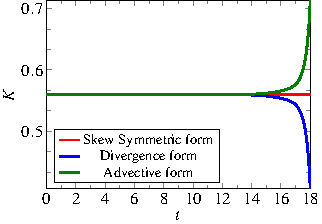
\includegraphics[width=0.41\textwidth]{./TikzFigures/thesis-figure0}
	}
	\subfloat[\label{p4.singular_values_decay}]{%
			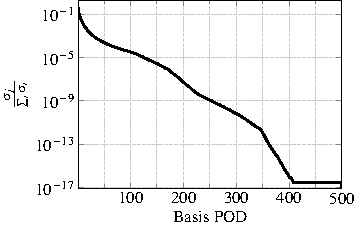
\includegraphics[width=0.45\textwidth]{./TikzFigures/thesis-figure1}
	} 
	\caption{\protect\subref{p4.compare_different_models} The kinetic energy $K$ for the advective, divergence and the skew-symmetric formulations. \protect\subref{p4.singular_values_decay} The decay of the singular values for the vortex merging.}
	\label{p4.fig:unstable_full_models}
	\end{centering}
\end{figure}

A total of $5000$ temporal snapshots is used to construct a reduced basis, following \Cref{alg:3.2}. The decay of the singular values, used as an indication of the reducibility of the problem, is presented in \Cref{p4.singular_values_decay}. The first $35$ POD modes correspond to over $99\%$ of the modes of the high fidelity solution. This suggests that an accurate reduced system can be constructed using a small number of basis vectors. To illustrate the effectiveness of the method, smaller bases are also considered.

For a qualitative analysis, in Figure \ref{p4.fig:snap_solution_incompressible_Euler}, four solutions at different times are shown for the high fidelity system and the reduced system with $k=17$ and $k=35$ modes. The overall dynamics of the problem, and in particular the formation and development of vorticity filaments, are correctly represented, even with a moderate number of basis vectors. Although small details are not captured by the reduced system with a small number of basis vectors, the position and the spreading of the vortices are comparable.

\begin{figure}[t]
\centering
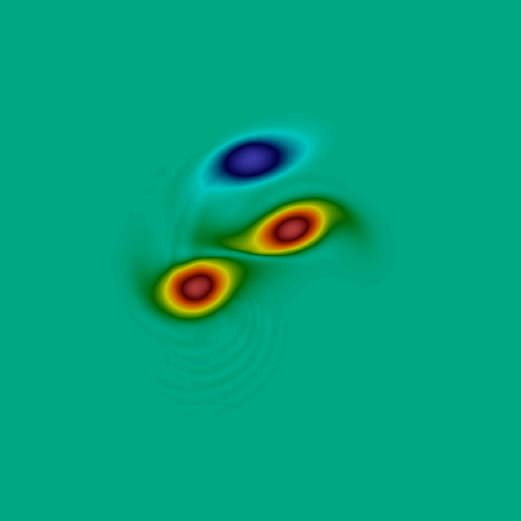
\includegraphics[scale=0.06]{data/Incompressible_Euler/Snapshots/red_17_2.png}\hspace{1em}
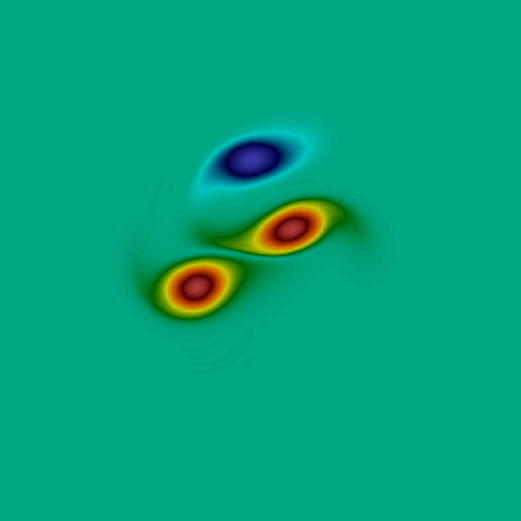
\includegraphics[scale=0.06]{data/Incompressible_Euler/Snapshots/red_35_2.png}\hspace{1em}
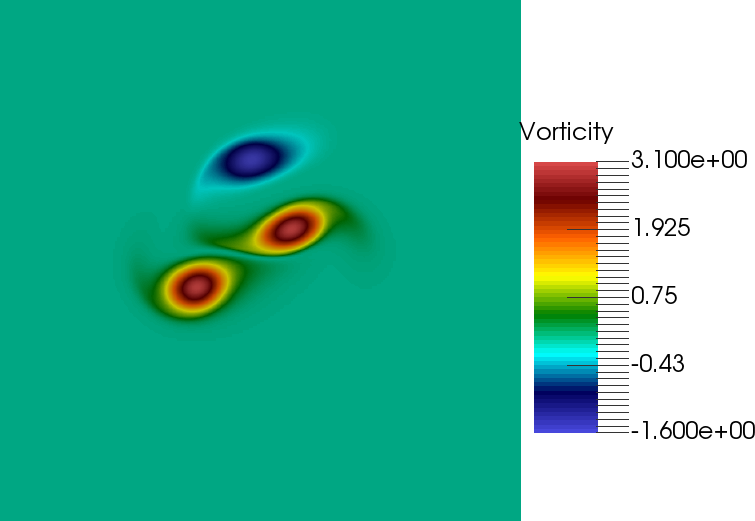
\includegraphics[scale=0.06]{data/Incompressible_Euler/Snapshots/Full_2.png}\\

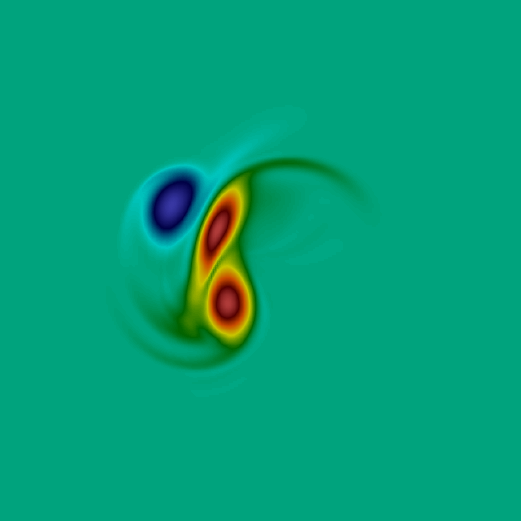
\includegraphics[scale=0.06]{data/Incompressible_Euler/Snapshots/red_17_3.png}\hspace{1em}
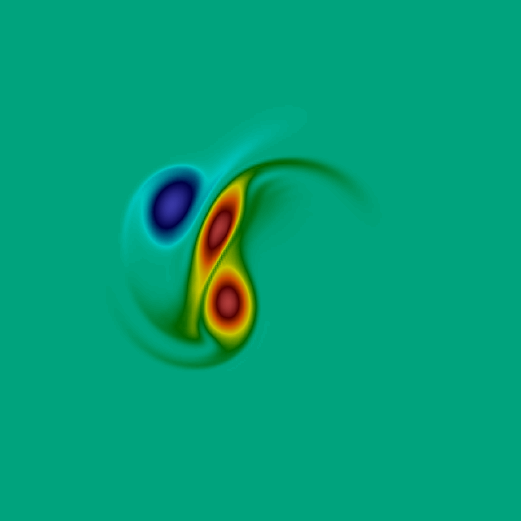
\includegraphics[scale=0.06]{data/Incompressible_Euler/Snapshots/red_35_3.png}\hspace{1em}
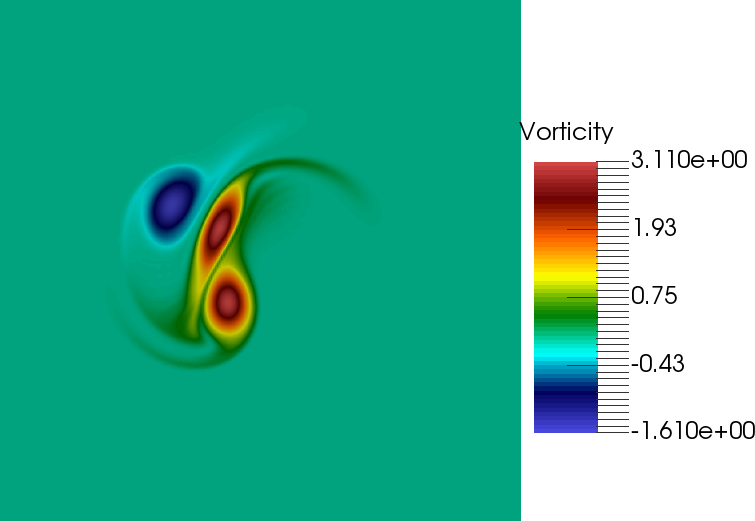
\includegraphics[scale=0.06]{data/Incompressible_Euler/Snapshots/Full_3.png}\\

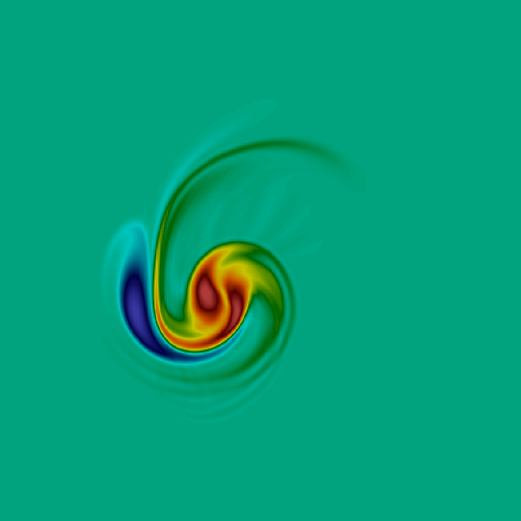
\includegraphics[scale=0.06]{data/Incompressible_Euler/Snapshots/red_17_4.png}\hspace{1em}
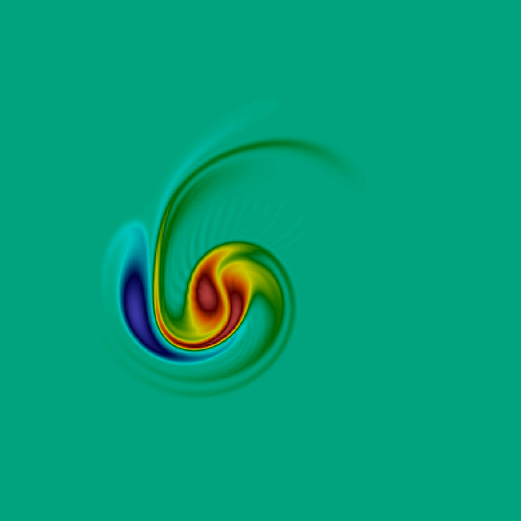
\includegraphics[scale=0.06]{data/Incompressible_Euler/Snapshots/red_35_4.png}\hspace{1em}
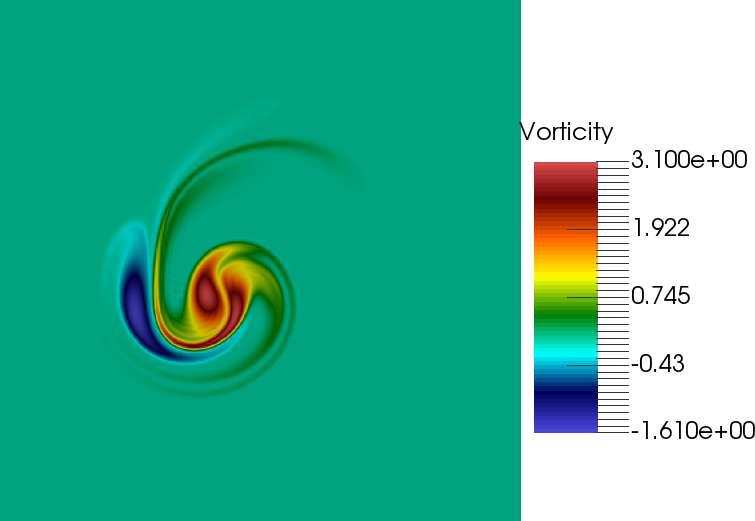
\includegraphics[scale=0.06]{data/Incompressible_Euler/Snapshots/Full_4.png}\\

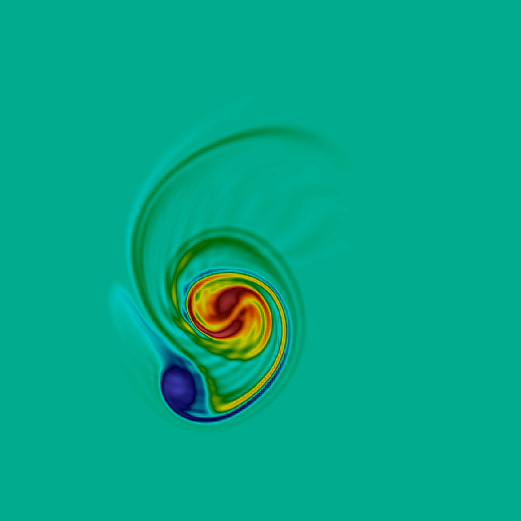
\includegraphics[scale=0.06]{data/Incompressible_Euler/Snapshots/red_17_5.png}\hspace{1em}
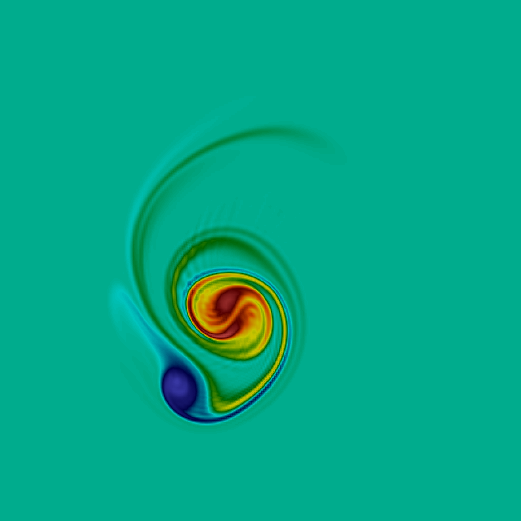
\includegraphics[scale=0.06]{data/Incompressible_Euler/Snapshots/red_35_5.png}\hspace{1em}
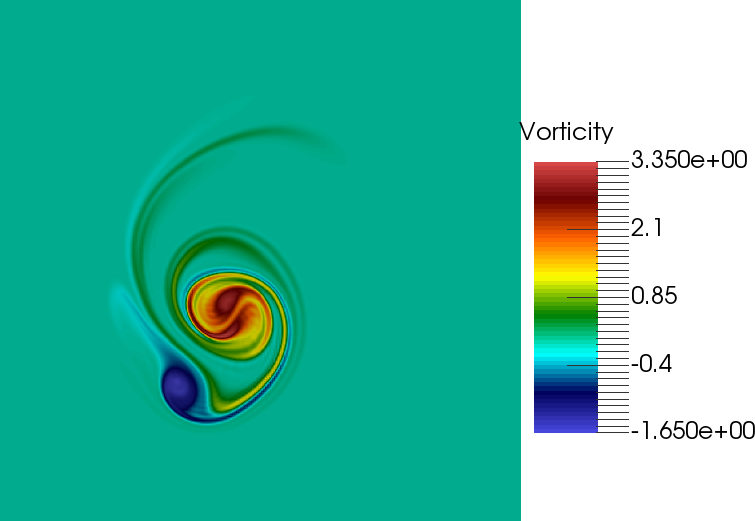
\includegraphics[scale=0.06]{data/Incompressible_Euler/Snapshots/Full_5.png}

\caption{Snapshots of the high-fidelity system and the reduced system at $t=\left\{ 4,8,12,18 \right\}$. From left to right: the solution of the reduced model with $k=17$, $k=35$ and the high fidelity solution.}
\label{p4.fig:snap_solution_incompressible_Euler}
\end{figure}

%%%%%%%%%%%%%%%%%%%%%%%%%%%%%%%%%%%%%%%%%%
%%%%%%%%%% Singular values decay merging vorteces %%%%%%%%%%%
%%%%%%%%%%%%%%%%%%%%%%%%%%%%%%%%%%%%%%%%%%
\Cref{p4.fig:approx_error_incompressible_Euler} shows the $L^2$ error between the high-fidelity solution and the reduced solution. The error decreases, consistently, as the number of basis vectors increases. Furthermore, the accuracy is maintained over the period of time integration.

The conservation of the kinetic energy is presented in \Cref{p4.fig:energy_error_incompressible_Euler}. Even for a small number of basis vectors, where the solution is not well approximated, the kinetic energy remains constant. Furthermore, the error in the kinetic energy, due to MOR, is constant in time. This is central for the robustness of the reduced system during long time-integration.


%%%%%%%%%%%%%%%%%%%%%%%%%%%%%%%%%%%%%%%%%%%
%%%%%%%%%% Approximation error and energy conservation %%%%%%%%%%
%%%%%%%%%%%%%%%%%%%%%%%%%%%%%%%%%%%%%%%%%%%
\begin{figure} [t]
	\begin{centering}
	\subfloat[\label{p4.fig:approx_error_incompressible_Euler}]{%
		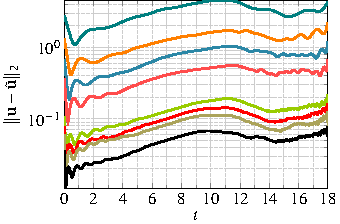
\includegraphics[width=0.41\textwidth]{./TikzFigures/thesis-figure2}
	}
	\subfloat[\label{p4.fig:energy_error_incompressible_Euler}]{%
			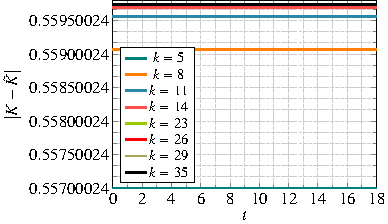
\includegraphics[width=0.45\textwidth]{./TikzFigures/thesis-figure3}
	} 
	\caption{\protect\subref{p4.fig:approx_error_incompressible_Euler} Evolution of $L_2$ error in velocity, between the high-fidelity system and the reduced system. \protect\subref{p4.fig:energy_error_incompressible_Euler} Conservation of the kinetic energy.}
	\label{p4.fig:energy_approx_err}
	\end{centering}
\end{figure}

\subsection{2D Kelvin-Helmholtz instability}
Consider the 2-dimensional compressible Euler equation \eqref{p4.eq:3.18} in a periodic square box $[0,1]^2$. Unlike the incompressible example in \Cref{p4.sec:res.1}, a centered finite difference scheme of fourth order is used to discretize \eqref{p4.eq:3.18}. The physical domain is discretized into a grid of $256\times 256$ nodes.

The initial conditions are given by
\begin{equation*}
\begin{cases}
& \mathbf{r} = 
\begin{cases}
& 2, \text{ if } 0.25<y<0.75,\\
& 1, \text{ otherwise },
\end{cases}
\\
& \mathbf{u}_x = a \sin(4\pi y) \left( e^{-\dfrac{(y-0.25)^2}{2\sigma^2}} + e^{-\dfrac{(y-0.75)^2}{2\sigma^2}} \right),\\
& \mathbf{u}_y = 
\begin{cases}
& 0.5, \text{ if } 0.25<y<0.75,\\
& -0.5, \text{ otherwise },
\end{cases},
\\
& \mathbf{p} = 2.5,\\
\end{cases}
\end{equation*}
where $a=0.1$ and $\sigma=5\sqrt{2}\cdot 10^{-3}$. This corresponds to contacting streams of fluid with different densities. For specific choices of parameters describing the jets, fine structures and vortices emerges at the interface between the streams. Such an instability is referred to as the Kelvin-Helmholtz instability \cite{HHS}.

As centered schemes are often dissipation free, resolving the discontinuous initial data requires some artificial viscosity. In the high-fidelity model, the method discussed in \cite{artificial_dissipation} is used as an artificial viscosity. However, at the level of the reduced system, this is replaced with a low pass filter on the expansion coefficients of POD basis vectors.

The fully discrete skew-symmetric form \eqref{p4.eq:3.27} is used as a time marching scheme with $\Delta t = 5 \cdot 10^{-4}$ over a period of $1$ time unit.

\Cref{p4.fig:error_decay_KH} illustrates that the accuracy of the method consistently improves as a higher number of POD basis modes are considered. Furthermore, the skew-symmetric form preserves the accuracy over the period of time integration. It is observed in \Cref{p4.fig:snap_solution_KH} that all features of the flow are correctly represented in the reduced system, even with a low number of basis vectors.

\begin{figure}[t]
\centering
	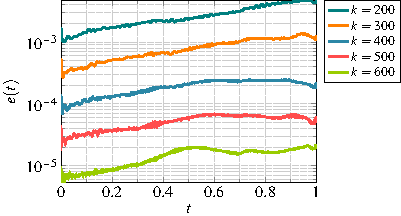
\includegraphics[width=0.5\textwidth]{./TikzFigures/thesis-figure4}
\caption{Evolution in time of the error  between the high fidelity solution of the Kelvin-Helmoltz and the reduced solution for different number of basis $k$. As error measure we use $e(t)=\sqrt{\|\mathbf{r}-\mathbf{r}^r\|^2+\|\mathbf{u_xr}-\mathbf{u_xr}^r\|^2 + \|\mathbf{u_yr}-\mathbf{u_yr}^r\|^2 + \|\mathbf{p}-\mathbf{p}^r\|^2}$.}
\label{p4.fig:error_decay_KH}
\end{figure}

Conservation of mass, momentum and energy is presented in \Cref{p4.fig:conservation_DEIM}. The accuracy of the method in approximating these invariants improves as the size of the basis is increased. Furthermore, \Cref{p4.energy_error_KH} shows how the kinetic energy associated with the reduced system mimic the kinetic energy of the high-fidelity system. This helps to ensure the correct evolution of kinetic energy, and thus, the internal energy.

\begin{figure} [t]
	\begin{centering}
	\subfloat[\label{p4.mass_error_KH}]{%
		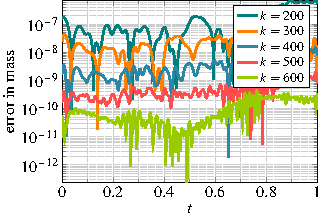
\includegraphics[width=0.45\textwidth]{./TikzFigures/thesis-figure5}
	}
	\subfloat[\label{p4.momentum_error_KH}]{%
			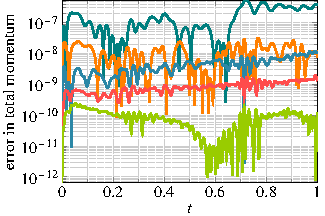
\includegraphics[width=0.45\textwidth]{./TikzFigures/thesis-figure6}
	} \\
	\subfloat[\label{p4.energy_error_KH}]{%
			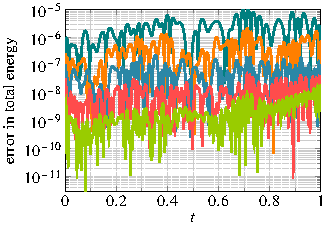
\includegraphics[width=0.45\textwidth]{./TikzFigures/thesis-figure7}
	}
	\caption{Difference between the high fidelity solution of the Kelvin-Helmholtz problem and the reduced solution of the mass \protect\subref{p4.mass_error_KH}, the momentum \protect\subref{p4.momentum_error_KH}, and the total energy \protect\subref{p4.energy_error_KH}.}
	\label{p4.fig:conservation_DEIM}
	\end{centering}
\end{figure}

%%%%%%%%%%%%%%%%%%%%%%%%%%%%%%%%%%%%%
%%%%%%%%%%%%%% Snapshots of KH %%%%%%%%%%%%%%
%%%%%%%%%%%%%%%%%%%%%%%%%%%%%%%%%%%%%
\begin{figure}[h!]
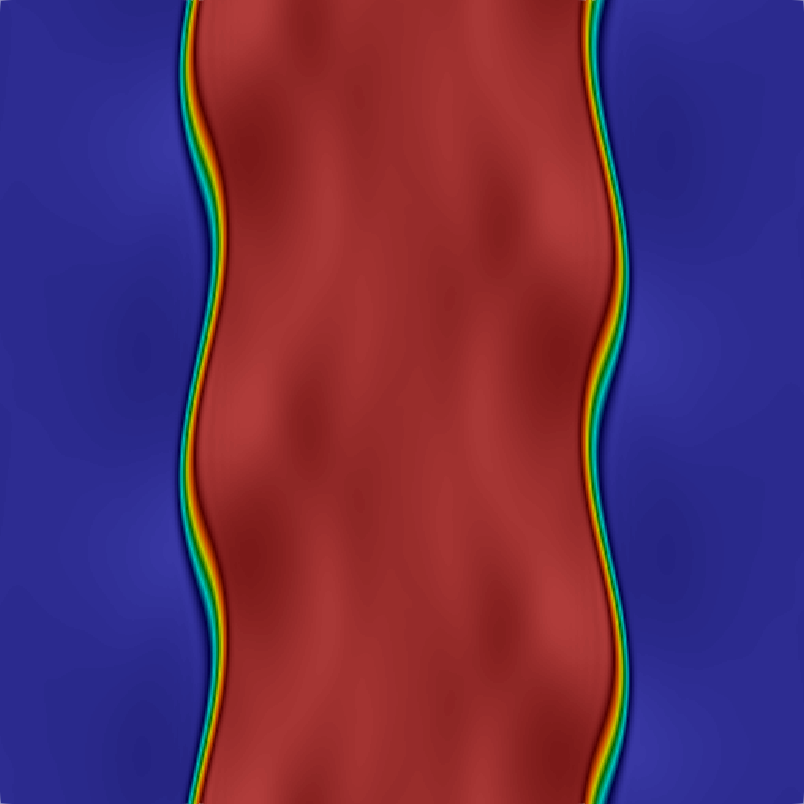
\includegraphics[scale=0.115]{data/Compressible_Euler/KH/Snapshots/density_200_307.png}\hspace{1em}
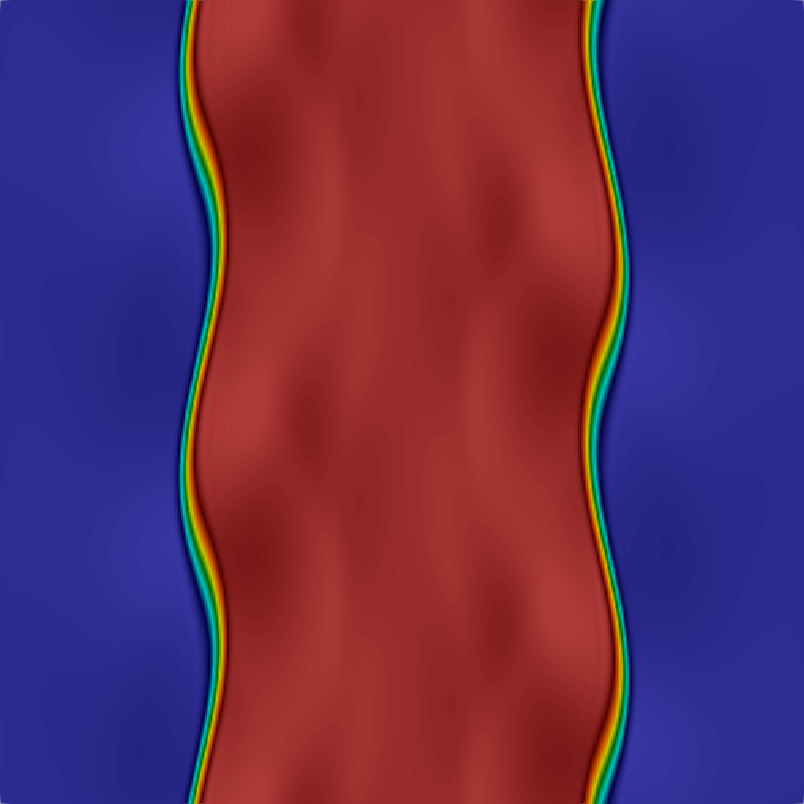
\includegraphics[scale=0.115]{data/Compressible_Euler/KH/Snapshots/density_500_307.png}\hspace{1em}
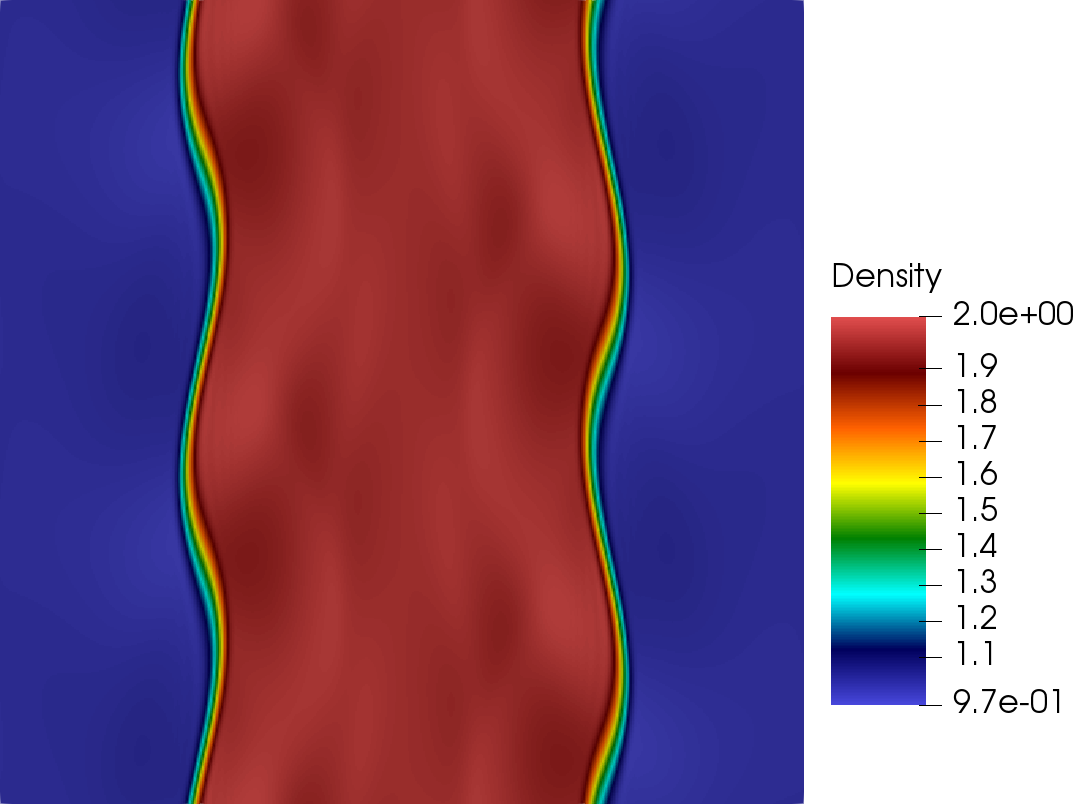
\includegraphics[scale=0.115]{data/Compressible_Euler/KH/Snapshots/density_exact_307.png}\\

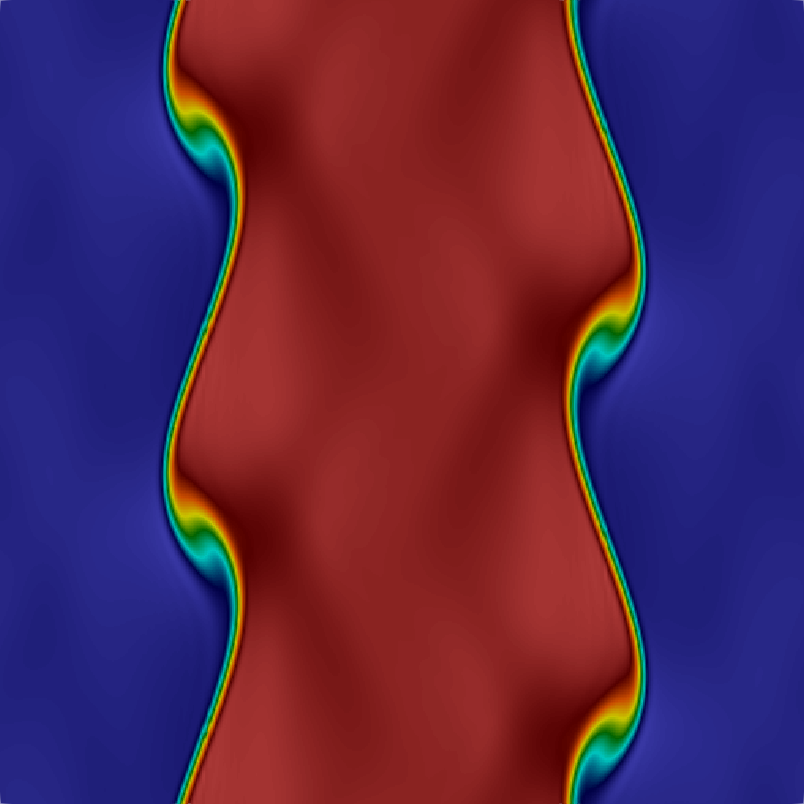
\includegraphics[scale=0.115]{data/Compressible_Euler/KH/Snapshots/density_200_461.png}\hspace{1em}
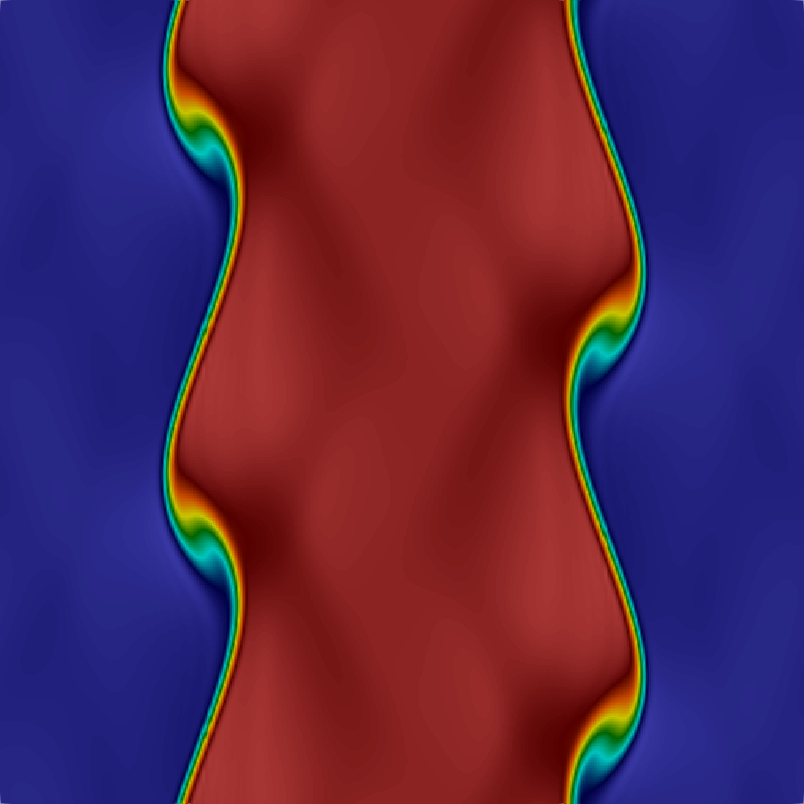
\includegraphics[scale=0.115]{data/Compressible_Euler/KH/Snapshots/density_500_461.png}\hspace{1em}
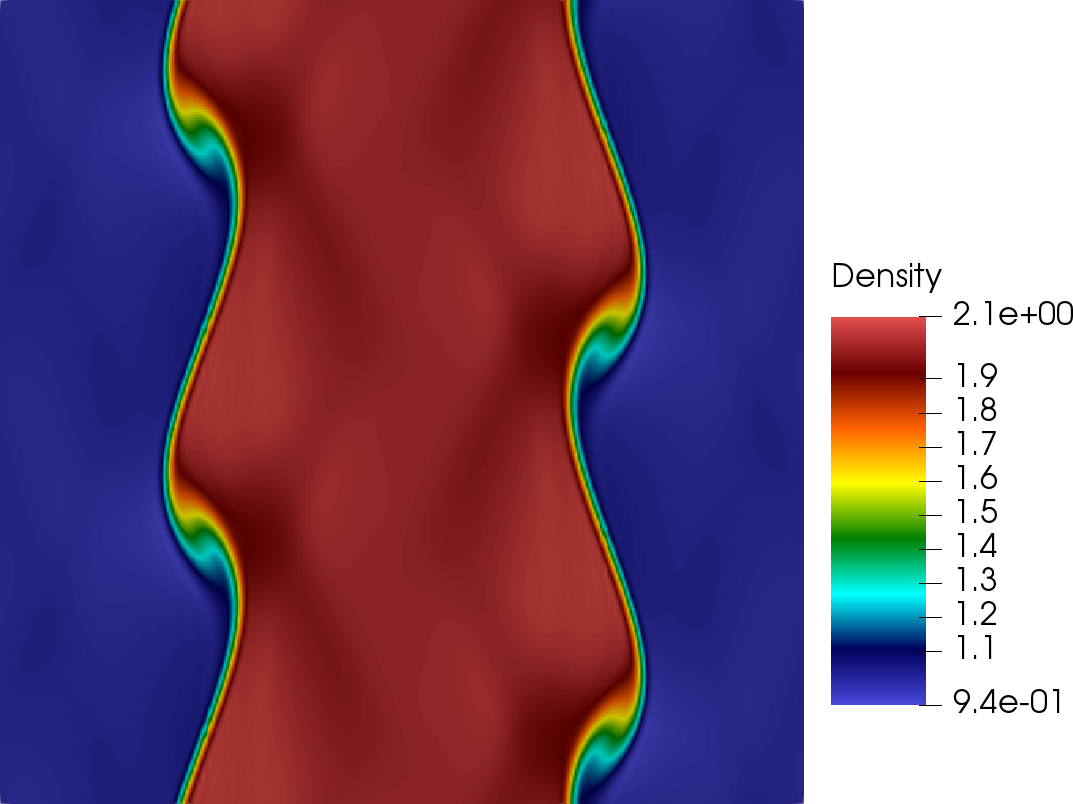
\includegraphics[scale=0.115]{data/Compressible_Euler/KH/Snapshots/density_exact_461.png}\\

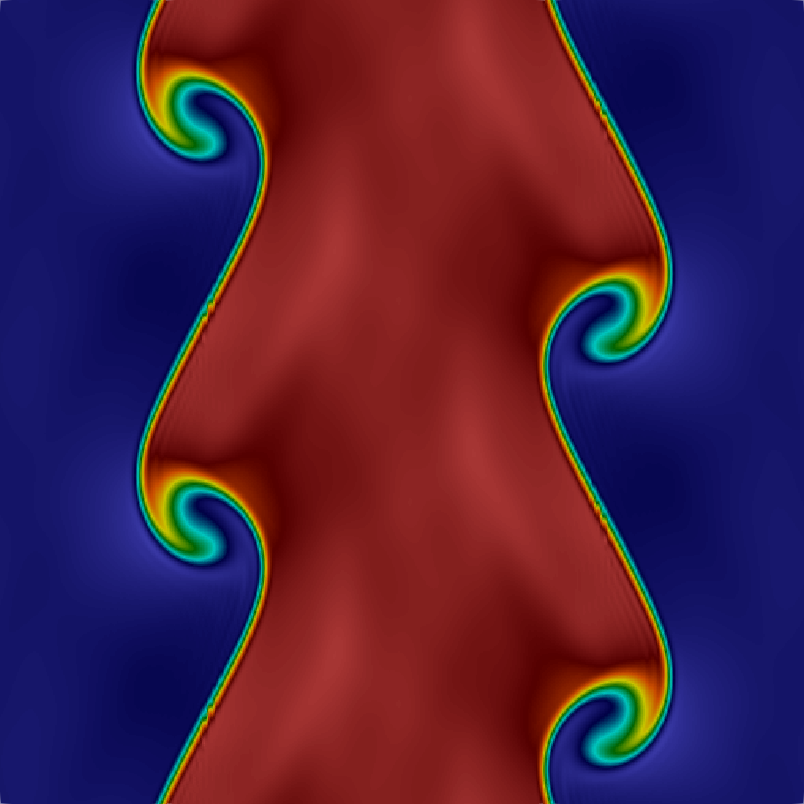
\includegraphics[scale=0.115]{data/Compressible_Euler/KH/Snapshots/density_200_614.png}\hspace{1em}
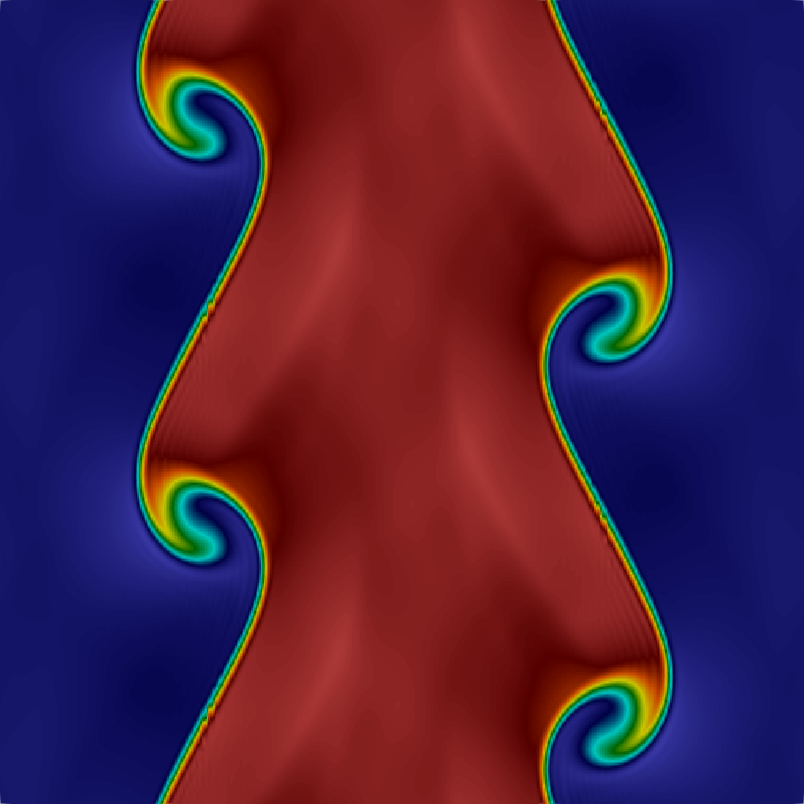
\includegraphics[scale=0.115]{data/Compressible_Euler/KH/Snapshots/density_500_614.png}\hspace{1em}
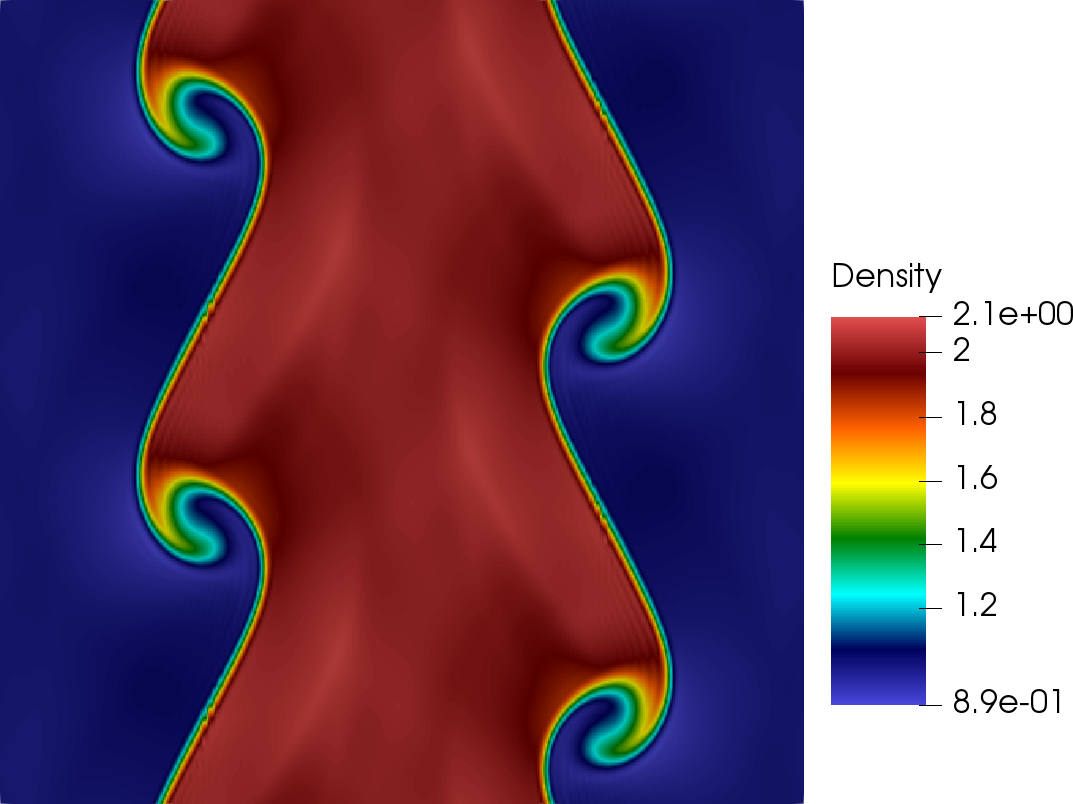
\includegraphics[scale=0.115]{data/Compressible_Euler/KH/Snapshots/density_exact_614.png}\\

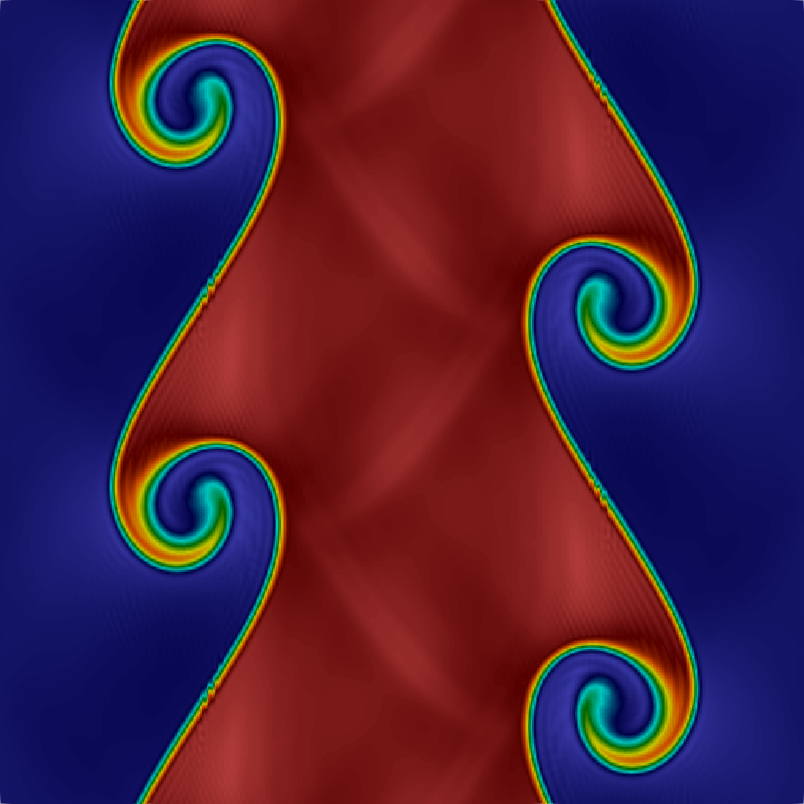
\includegraphics[scale=0.115]{data/Compressible_Euler/KH/Snapshots/density_200_768.png}\hspace{1em}
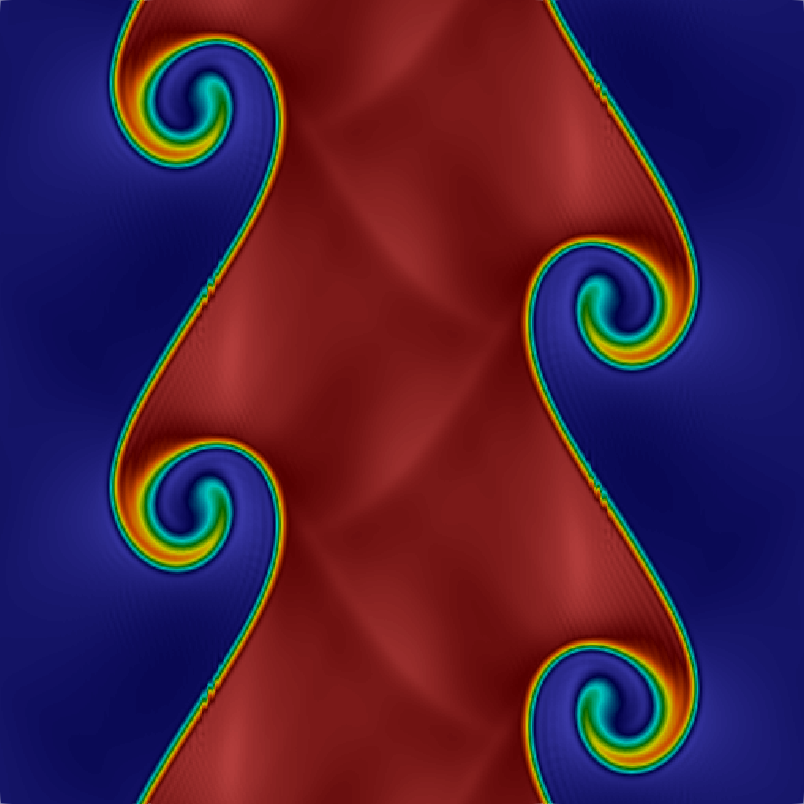
\includegraphics[scale=0.115]{data/Compressible_Euler/KH/Snapshots/density_500_768.png}\hspace{1em}
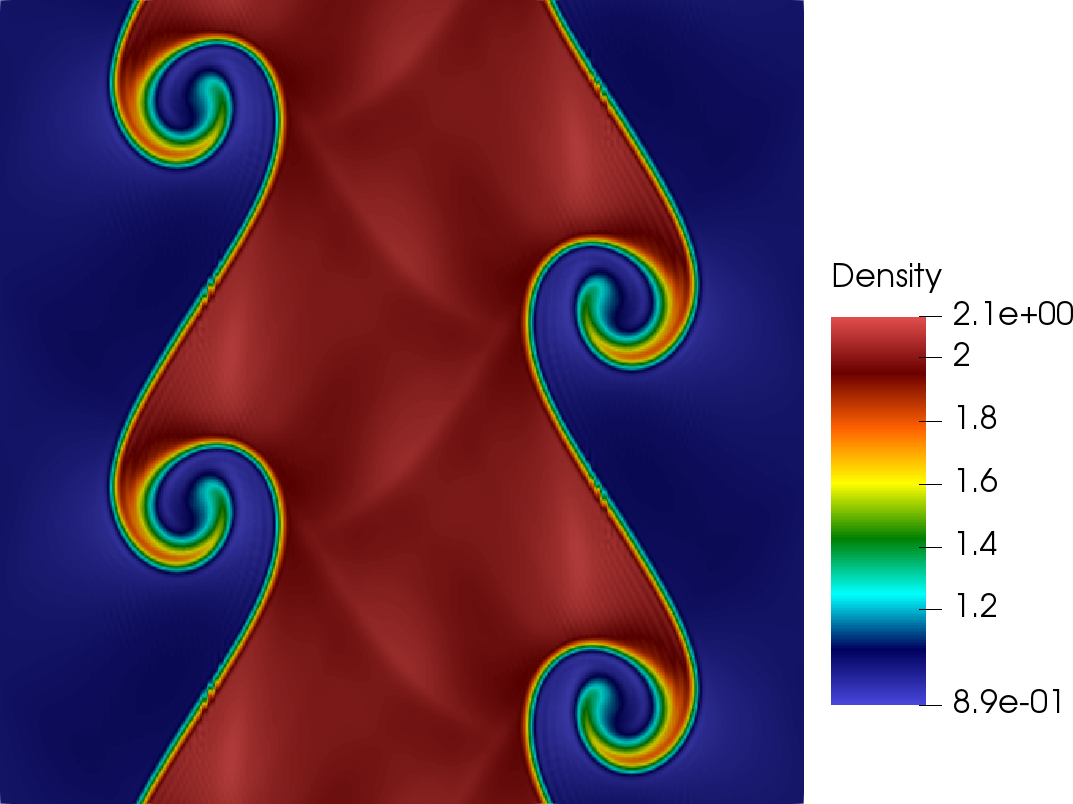
\includegraphics[scale=0.115]{data/Compressible_Euler/KH/Snapshots/density_exact_768.png}

\caption{Solutions of the Kelvin-Helmholtz problem at $t=\left\{ 0.4, 0.6, 0.8, 1 \right\}$. From left to right we show the solution of the reduced model with $k=200$, $k=500$ and the high fidelity solution.}
\label{p4.fig:snap_solution_KH}
\end{figure}


\subsection{1D Shock problem} \label{sec:p4.res.3}
In this section we study the 1-dimensional compressible Euler problem, \eqref{p4.eq:3.18} without viscous terms, with a steady state discontinuous solution. This is in preparation for \Cref{p4.sec:5.res.4}, where development and propagation of shock waves is discussed. Here we asses how the skew-symmetric form of \eqref{p4.eq:3.18} can recover moving discontinuities at the level of the reduced system. Consider a periodic boundary conditions on $\Omega = [0,1]$ with the initial condition
\begin{equation*}
\begin{cases}
& \mathbf{r} = 0.5+0.2 \cos(2\pi x),\\
& \mathbf{u} = 1.5,\\
& \mathbf{p} = 0.5+0.2 \sin(2\pi x).\\
\end{cases}
\end{equation*}
The domain is discretized into $N=2000$ nodes and a centered finite differences scheme is used to assemble the discrete Euler equation in skew-symmetric form, as discussed in \Cref{p4.sec:skew.3}. 

The fully discrete skew-symmetric form \eqref{p4.eq:3.27} is used for time integration over a time interval $[0,0.3]$. To resolve the discontinuous solution we use an artificial viscosity with $\tau = \mu \partial u / \partial x$, where $\mu = 0.5 \cdot 10^{-4}$.

\Cref{p4.fig:energy_pres_1D} shows the evolution of conserved quantities for the high-fidelity and reduced system. Here, the high-fidelity model is also considered in the divergence and advective form in addition to the skew-symmetric form. It is clear that when the reduced systems is not in skew-symmetric form, it violates conservation of mass, momentum, and energy. Even while the high-fidelity systems in divergence and advective forms are stable, the constructed reduced system is unstable, independently by the number of basis vectors. On the other hand, the skew-symmetric form yields a stable and conservative reduced system. Note that the loss in the energy associated with the skew-symmetric form, illustrated in \Cref{p4.conservation_1D_focus.b,p4.conservation_1D_focus.d,p4.conservation_1D_focus.f}, is due to the application of an artificial viscosity. 

\Cref{p4.error_behaviour_1D} shows the total error, when the reduced system captures a discontinuous solution at $t=0.16$. It is observed that the formation of a discontinuity affects the accuracy of the method. This is expected as a sharp gradient is approximated by a relatively few POD modes. However, the method remains robust and stable during the period of time integration.

In \Cref{p4.fig:snaps_1D_Euler} we compare the numerical artifacts of different formulations of the Euler equation. The advective formulation is not presented since it does not yield a stable reduced system. It is observed that the reduced system based on the skew-symmetric formulation accurately represent the overall behavior of the high-fidelity solution. On the other hand, a Gibbs-type error \cite{thompson1992fourier} appears near sharp gradients, for the reduced system based on the divergence form of the Euler equation. The well-representation of the skew-symmetric form is due the low aliasing error property. 

As discussed in \Cref{p4.sec:mor_skew}, the DEIM approximation needed for an efficient evaluation of the nonlinear components of \eqref{p4.eq:3.18}, can affect the conservation properties of the skew-symmetric form. \Cref{p4.fig:singular_values_decay_1D} shows the decay of the singular values of the nonlinear snapshots. The decay of these snapshots is significantly slower than the temporal snapshots of \eqref{p4.eq:3.18}. This indicates that to maintain the accuracy of the reduced system, the DEIM basis should be chosen richer than the POD basis. \Cref{p4.error_DEIM} and \Cref{p4.energy_DEIM} present the error and the conservation of total energy when the DEIM is used to approximate the nonlinear term. The conservation of energy is recovered once DEIM approximates the nonlinear terms with enough accuracy. 
In this numerical experiment, evaluation of the nonlinear terms in \eqref{p4.eq:3.18} using the DEIM is ten times faster than the high-fidelity evaluation.

\begin{figure} [h!]
	\begin{centering}
	\subfloat[\label{p4.conservation_1D.a}]{%
		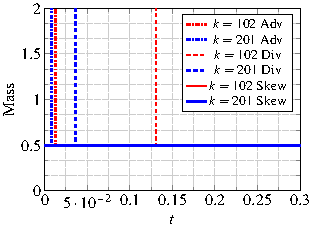
\includegraphics[width=0.40\textwidth]{./TikzFigures/thesis-figure8}
	}
	\subfloat[\label{p4.conservation_1D_focus.b}]{%
			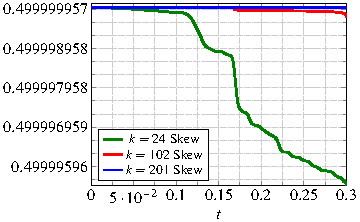
\includegraphics[width=0.45\textwidth]{./TikzFigures/thesis-figure9}
	} \\
	\subfloat[\label{p4.conservation_1D.c}]{%
			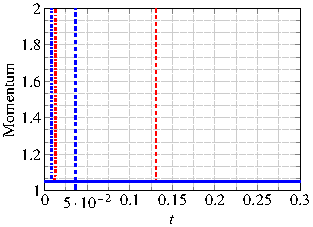
\includegraphics[width=0.40\textwidth]{./TikzFigures/thesis-figure10}
	}
	\subfloat[\label{p4.conservation_1D_focus.d}]{%
			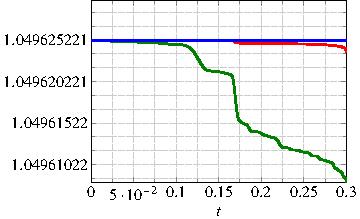
\includegraphics[width=0.45\textwidth]{./TikzFigures/thesis-figure11}
	} \\
	\subfloat[\label{p4.conservation_1D.e}]{%
			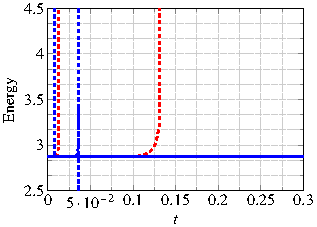
\includegraphics[width=0.40\textwidth]{./TikzFigures/thesis-figure12}
	}
	\subfloat[\label{p4.conservation_1D_focus.f}]{%
			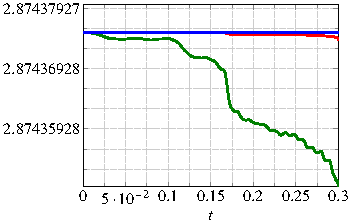
\includegraphics[width=0.45\textwidth]{./TikzFigures/thesis-figure13}
	}
	\caption{ (left)  Evolution of the three conserved quantities for the reduced solution of the compressible Euler equation (mass, total momentum and total energy).  The divergent, advective and skew-symmetric formulations have been considered and $k=102,204$ basis are used in the reduced model. (right) Evolution of the conserved quantity for a stable reduced model using the skew-symmetric formulation.}
	\label{p4.fig:energy_pres_1D}
	\end{centering}
\end{figure}

\begin{figure}[h!]
\centering
	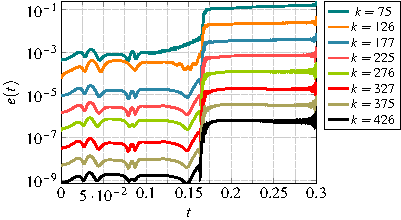
\includegraphics[width=0.5\textwidth]{./TikzFigures/thesis-figure14}
\caption{Evolution in time of the error  between the high fidelity solution of the 1D compressible Euler and the reduced solution for different number of basis $k$. As error measure we consider $e(t)=\sqrt{\|\mathbf{r}-\mathbf{r}^r\|^2+\|\mathbf{ur}-\mathbf{ur}^r\|^2+\|\mathbf{p}-\mathbf{p}^r\|^2}$.}
\label{p4.error_behaviour_1D}
\end{figure}

\begin{figure} [h!]
	\begin{centering}
	\subfloat[\label{p4.fig:snaps_1D_Euler.a}]{%
		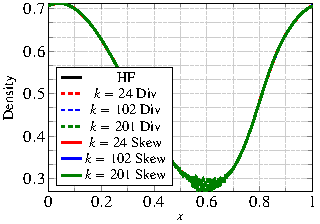
\includegraphics[width=0.45\textwidth]{./TikzFigures/thesis-figure15}
	}
	\subfloat[\label{p4.fig:snaps_1D_Euler.b}]{%
			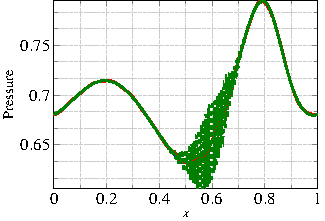
\includegraphics[width=0.45\textwidth]{./TikzFigures/thesis-figure16}
	} \\
	\subfloat[\label{p4.fig:snaps_1D_Euler.c}]{%
			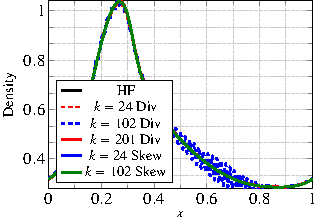
\includegraphics[width=0.45\textwidth]{./TikzFigures/thesis-figure17}
	}
	\subfloat[\label{p4.fig:snaps_1D_Euler.d}]{%
			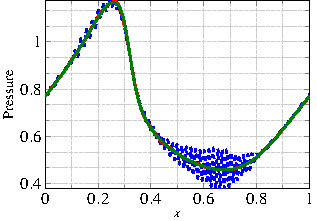
\includegraphics[width=0.45\textwidth]{./TikzFigures/thesis-figure18}
	} \\
	\subfloat[\label{p4.fig:snaps_1D_Euler.e}]{%
			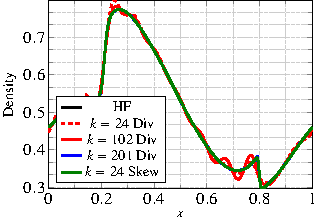
\includegraphics[width=0.45\textwidth]{./TikzFigures/thesis-figure19}
	}
	\subfloat[\label{p4.fig:snaps_1D_Euler.f}]{%
			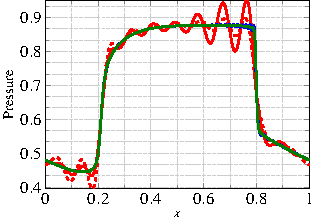
\includegraphics[width=0.45\textwidth]{./TikzFigures/thesis-figure20}
	}
	\caption{Qualitative comparison between different formulations for the reduced model in terms of density (left) and pressure (right) at $t=0.1,0.3$ and $1$s. Results for the advective formulation are not showed here because the related reduced solutions are unstable after a few time steps.}
	\label{p4.fig:snaps_1D_Euler}
	\end{centering}
\end{figure}

\begin{figure}[h!]
\centering
	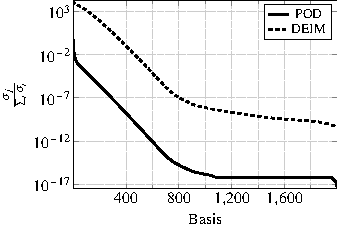
\includegraphics[width=0.5\textwidth]{./TikzFigures/thesis-figure21}
\caption{Decay of the singular values of the snapshot matrix related to POD and DEIM algorithms for the 1D compressible Euler problem.}
\label{p4.fig:singular_values_decay_1D}
\end{figure}

\begin{figure} [h!]
	\begin{centering}
	\subfloat[\label{p4.error_DEIM}]{%
		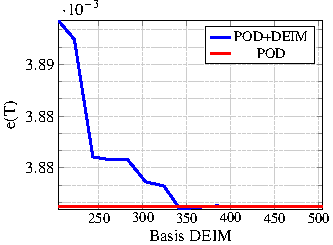
\includegraphics[width=0.45\textwidth]{./TikzFigures/thesis-figure22}
	}
	\subfloat[\label{p4.energy_DEIM}]{%
			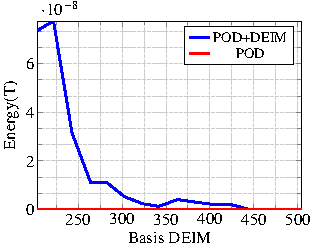
\includegraphics[width=0.425\textwidth]{./TikzFigures/thesis-figure23}
	} 
	\caption{Comparison between standard POD and POD with DEIM treatment of the nonlinear term in terms of the error \protect\subref{p4.error_DEIM} and the total energy \protect\subref{p4.energy_DEIM}.}
	\label{p4.fig:RIC2}
	\end{centering}
\end{figure}

\subsection{Continuous Variable Resonance Combustor} \label{p4.sec:5.res.4}

CVRC is a model rocket combustor, designed and operated at Purdue University (Indiana, U.S.) to investigate combustion instabilities \cite{yu2008combustion}. This setup is called the Continuously Variable Resonance Combustor (CVRC) because the length of the oxidizer injector can be varied continuously, allowing for a detailed investigation of the coupling between acoustics and combustion in the chamber \cite{garby2013simulations}. The 2D/3D high-fidelity simulations of CVRC are expensive. Thus to get a fast analysis tool, a quasi-1D model has been proposed by Smith et al. \cite{smith2008computational} and further developed by Frezzotti et al. \cite{frezzotti2015determination,frezzotti2017numerical,frezzotti2018quasi}. 


The CVRC consists of three parts: oxidizer post, combustion chamber and exit nozzle, as shown in Fig. \ref{p4.fig:radius}. The oxidizer is injected from the left end of the oxidizer post and meets the fuel, injected through an annular ring around the oxidizer injector, at the back-step. The combustion happens in a region around the back-step. The combustion products flow through the chamber and exit the system from the nozzle.  Both the injector and the nozzle are operated at choked condition during the experiment. The length of the oxidizer post $L_{op}$ of the CVRC can be varied continuously, leading to different dynamics. Here, we focus on the case with $L_{op}= 14.0$ cm, in which the combustion is unstable.

The geometry parameters of the quasi-1D CVRC with a oxidizer post length  $L_{op}= 14.0$ cm are shown in \Cref{p4.tab:geometry_parameters}.  The back-step and the converging part of the nozzle are sinusoidally contoured to avoid a discontinuity of the radius that will invalidate the quasi-1D governing equations presented in the next subsection.

\begin{figure}[h!]
\centering
	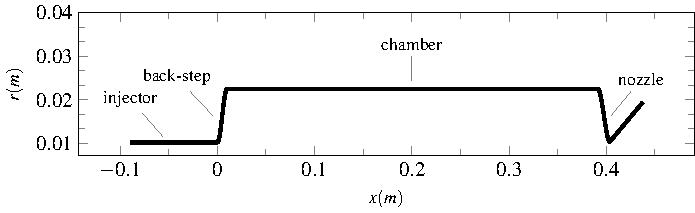
\includegraphics[width=0.9\textwidth]{./TikzFigures/thesis-figure24}
\caption{Geometry of quasi-1D CVRC model.}
\label{p4.fig:radius}
\end{figure}

\begin{table} [h]
	\centering
	\caption{Geometry parameters of the quasi-1D CVRC with an oxidizer post length $L_{op}=14$ cm.}
	\centering
	\begin{tabular}{c c c c c c }
		\toprule
		\centering
		\multirow{2}{*}{Section} &
		\multicolumn{2}{c}{Oxidizer post} &
		\multirow{2}{*}{Chamber} &
		\multicolumn{2}{c}{Nozzle} \\
		\cmidrule(lr){2-3} \cmidrule(lr){5-6}
		& injector & back-step & & converging part & diverging part\\
		\midrule
		Length (cm) & 12.99 & 1.01 & 38.1 & 1.27 & 3.4 \\
		Radius (cm) & 1.02  & $1.02 \sim 2.25$ & 2.25 & $2.25 \sim 1.04$ & $1.04 \sim 1.95$ \\
		\bottomrule
		\label{p4.tab:geometry_parameters}
	\end{tabular} 
\end{table}
The fuel is pure gaseous methane. The oxidizer is a mixture of 42\% oxygen and 58\% water (per unit mass), and is injected in the oxidizer post at a temperature $T_{ox}=1030\text{K}$ so that both water and oxygen are in the gaseous phase. The operating conditions are listed in Table \ref{p4.tab:operating-conditions}.

\begin{table} [h]
	\centering
	\caption{CVRC operating conditions.}
	\centering
	\begin{tabular}{l l l}
		\toprule
		\centering
		Parameter & Unit & Value \\
		\midrule
		Fuel mass flow rate, $\dot{m}_{f}$ & kg/s & 0.027   \\
		Fuel temperature, $T_{f}$ & K & 300   \\
		Oxidizer mass flow rate, $\dot{m}_{ox}$ & kg/s & 0.32   \\
		Oxidizer temperature, $T_{ox}$ & K & 1030   \\
		$O_2$ mass fraction in oxidizer, $Y_{O_2}$ & -- & 42.4\%   \\
		$H_2O$ mass fraction in oxidizer, $Y_{H_2O}$ & -- & 57.6\%   \\
		Mean chamber pressure & MPa & 1.34 \\
		Equivalence ratio, $E_r$ & -- & 0.8 \\
		\bottomrule
		\label{p4.tab:operating-conditions}
	\end{tabular} 
\end{table}
For the combustion, we consider the one-step reaction model
\begin{equation*}\label{p4.eq:combustion}
CH_4 + 2O_2 \rightarrow CO_2 + 2H_2O.
\end{equation*}
We assume that the fuel reacts instantaneously to form products, allowing us to neglect intermediate species and finite reaction rates. As the equivalence ratio is less than one, there is oxidizer left after the combustion. Therefore, only two species need to be considered: oxidizer and combustion products.


The governing equations that describe the conservation of mass, momentum, and energy of the quasi-1D CVRC flow, are the quasi-1D unsteady Euler equations for multiple species, expressed in conservative form as
\begin{equation}\label{p4.eq:5p2.1}
\frac{\partial }{\partial t} v + \frac{\partial }{\partial x} F_v = s_A + s_f + s_q.
\end{equation}
The conserved variable vector $v$ and the convective flux vector $F$ are
\begin{equation}\label{p4.eq:5p2.2}
v= \left( \begin{gathered}
\rho A  \\
\rho uA  \\
\rho EA  \\
\rho Y_{ox} A \\
\end{gathered} \right), 
F = \left( \begin{gathered}
\rho uA  \\
\left(\rho u^2 + p\right)A  \\
\left(\rho E + p\right)uA  \\
\rho uY_{ox} A \\
\end{gathered} \right),
\end{equation}
where $\rho$ is the density, $u$ is the velocity, $p$ is the pressure, $E$ is the total energy, $Y_{ox}$ is the mass fraction of oxidizer, and $A=A(x)$ is the cross sectional area of the duct. The pressure $p$ can be computed using the conserved variables as
\begin{equation}\label{p4.eq:total-engery}
E = \frac{p}{\rho (\gamma - 1)} + \frac{u^2}{2} - C_p T_{ref},
\end{equation}
where $T_{ref}$ is the reference temperature and is set as 298.15 K. The temperature $T$ is recovered from the equation of state $p = \rho R T$. The gas properties  $C_p$, $R$ and $\gamma$ are computed as $C_p= \sum C_{pi}Y_i$, $R=\sum R_iY_i$ and $ \gamma= C_p/(C_p-R)$, respectively. 

The source terms are
\begin{equation} \label{p4.eq:5p2.3}
s_A = \left( \begin{gathered}
0  \\
p \frac{dA}{dx}  \\
0  \\
0 \\
\end{gathered} \right), 
s_f = \left( \begin{gathered}
{\dot \omega}_f  \\
{\dot \omega}_f u  \\
{\dot \omega}_f \left(h_{0}^{f} + \Delta h_{0}^{rel} \right)  \\
{\dot \omega}_{ox} \\
\end{gathered} \right), 
{s_q} = \left( \begin{gathered}
0  \\
0  \\
q'  \\
0 \\
\end{gathered} \right),
\end{equation}
where $\dot{\omega}_f$ is the depletion rate of the fuel, $\dot{\omega}_{ox}$ is the depletion rate of the oxidizer, $h_0^f$ is the total enthalpy of the fuel, $\Delta h_{0}^{rel}$ is the heat of reaction per unit mass of fuel and $q'$ is the unsteady heat release term. $s_A$ accounts for area variations, $s_f$ and $s_q$ are related to the combustion. $s_f$ represents the addition of the fuel and its combustion with the oxidizer, which in turn results in the creation of the combustion products. The depletion rate of the fuel is
\begin{equation}\label{p4.eq:5p2.4}
\dot{\omega}_{f}= \frac{k_f \dot{m}_f Y_{ox} \left(1+sin\xi\right)}{l_f-l_s},
\end{equation} 
where
\begin{equation}\label{p4.eq:5p2.5}
\xi= -\frac{\pi}{2} + 2\pi\frac{x-l_s}{l_f-l_s}, \hspace{0.5cm} \forall \hspace{0.2cm} l_s < x < l_f.
\end{equation}
The setting of the fuel injection restricts the combustion to the region $l_s < x < l_f$. The reaction constant $k_f$ is selected to insure that the fuel is consumed within the specified combustion zone. The depletion rate of the oxidizer is computed by 
\begin{equation}\label{p4.eq:5p2.6}
\dot{\omega}_{ox} = C_{o/f} \dot{\omega}_f,
\end{equation}
where $C_{o/f}$ is the oxidizer-to-fuel ratio.

The unsteady heat release term $q'$, also called the combustion response function, models the coupling between acoustics and combustion. Here, we use the combustion response function designed by Frezzotti et al. \cite{frezzotti2017numerical,frezzotti2018quasi}, which is a function of the velocity, sampled at specific abscissa $\hat{x}$ that is almost coincident with the antinode of the first longitudinal modal shape with a time lag $t_0$, i.e.,
\begin{equation}\label{p4.eq:5p2.7}
q'\left( x,t\right) = \alpha g\left(x\right)  A\left(x\right) \left[ u\left( \hat{x},t-t_0 \right) - \bar{u}\left( \hat{x} \right) \right].
\end{equation}
Here $\bar{u}$ is the time averaged velocity, estimated with the steady-state quasi-1D model assuming $q'=0$, and $g(x)$ is a Gaussian distribution  
\begin{equation}\label{eq:5p2.8}
g\left(x\right)= \frac{1}{\sqrt{2\pi\sigma^2}} \exp\left( -\frac{\left(x-\mu\right)^2}{2\sigma^2} \right),
\end{equation}
where $\mu$ is the mean and $\sigma$ is the standard deviation. The amount of heat release due to velocity oscillations is controlled by the parameter $\alpha$, in \eqref{p4.eq:5p2.7}.

The boundary conditions for the quasi-1D CVRC flow include the fixed mass flow rate and the stagnation temperature at the head-end of the oxidizer injector, and the supersonic outflow at the exit of the nozzle.

Prior to the unsteady simulation, the quasi-1D CVRC needs to be excited, which is achieved by adding a perturbation to the steady-state solution. The perturbation is added by forcing the mass flow rate with a multi-sine signal
\begin{equation}\label{eq:5p2.9}
\dot{m}_{ox} \left(t\right)= \dot{m}_{ox,0} \left[1 + \delta\sum_{k=1}^{K}  sin\left(2\pi k\Delta f t\right) \right],
\end{equation}
where $\dot{m}_{ox,0}$ is the oxidizer mass flow rate in Table \ref{p4.tab:operating-conditions}, $\Delta f$ is the frequency resolution and $K$ is the number of frequencies. In this paper, $\Delta f = 50 $ Hz and $K=140$, resulting in a minimal frequency of 50 Hz and a maximal frequency of 7000 Hz. $\delta$ is required to be small to control the amplitude of the perturbation and is set as 0.1\%.

The procedure of the unsteady simulation of the quasi-1D CVRC flow includes three steps:
\begin{enumerate} [label={\arabic*.}]
	\item  Compute the steady-state solution by setting $\dot{m}_{ox}=\dot{m}_{ox,0} $ and $q'=0$.
	\item  Excite the system by adding a perturbation to the oxidizer mass flow rate according to (\ref{p4.eq:5p2.7}) and setting $q'=0$.
	\item  Perform the unsteady simulation by turning on the combustion response function $q'$ in (\ref{p4.eq:5p2.3}) and turning off the oxidizer mass flow rate perturbation by setting $\dot{m}_{ox}=\dot{m}_{ox,0} $.	
\end{enumerate}
Introduction of an artificial viscosity is essential for a robust and long time-integration of \eqref{p4.eq:5p2.3}. Common discretization schemes for \eqref{p4.eq:5p2.3} are often dissipative, e.g., the Lax-Friedrich scheme used in \cite{Wang:255719}. Since the skew-symmetric discretization is non-dissipative, we modify \eqref{p4.eq:5p2.3} as
\begin{equation} \label{p4.eq:5p2.10} 
	\frac{\partial }{\partial t} v + \frac{\partial }{\partial x} F = s_A + s_f + s_q + d, \quad d = (0,\frac{\partial }{\partial x} \tau,0,0)^T,
\end{equation}
with $\tau = \mu \partial (u A)/ \partial x$, and $\mu = 6\times 10^{-5}$. This type of artificial viscosity is chosen for its simplicity. This, however, can be replaced with a more moderate and sophisticated method. 

Note that the right hand side in \eqref{p4.eq:5p2.10} suggests that, in general, mass, momentum, and energy is not conserved. Furthermore, the complex coupling of the variables in \eqref{p4.eq:5p2.3} and the non-constant adiabatic gas index prohibit the application of complex and implicit time integration schemes. Therefore, a quasi-skew-symmetric form, introduced in \eqref{p4.eq:3.7}, is used for \eqref{p4.eq:5p2.3}. It is straight-forward to check \cite{sjogreen2010skew}, for $t,s\in \mathbb R^{N}$
\begin{equation} \label{p4.eq:5p2.9.1}
	\frac 1 2 \delta_x (st)_j + \frac 1 2 s_j \delta_x (t)_j + \frac 1 2 t_j \delta_x (s)_j = \frac 1 4 \delta_x^+( s_j + s_{j-1} )(t_j + t_{j-1}).
\end{equation}
where $\delta_x (v)_j = \left( v_{j+1} - v_{j-1} \right)/\Delta x$ is centered finite difference approximation of the space derivative and $\delta_x^+ (v_j) = \left( v_{j+1} - v_j \right) /\Delta x$, for some $v\in \mathbb R^{N}$. Therefore,
\begin{equation} \label{p4.eq:5p2.9.2}
	F_{i+1/2}^{\Delta}(s_jt_j,s_{j+1}t_{j+1}) = ( s_j + s_{j-1} )(t_j + t_{j-1}),
\end{equation}
can be interpreted as an approximation of a quadratic flux function at the boundary of two adjacent finite volume cells. A better approximation of the flux in \eqref{p4.eq:5p2.9.2} corresponds to a higher order skew-symmetric form for a quadratic variable $st$ in \eqref{p4.eq:5p2.9.1}. We discretize the real line into N uniform cells of size $\Delta x$. A quasi-skew-symmetric form for \eqref{p4.eq:5p2.10} now takes the form
\begin{equation}
\begin{aligned}
	\frac{d}{dt} q^i_j + \delta^+ F^{\Delta}_{i+1/2}(q^i_jr^i_j,q^i_{j+1}r^i_{j+1}) &- \delta^+ F_d^{\Delta}(d^i_j,d^i_{j+1}) + \delta^+ F_p^{\Delta}(p_j,p_{j+1}) \\
	&= \int_{c_j} s_A + s_f + s_q \ dx.
\end{aligned}
\end{equation}
for $j=1,\dots,N$. Here, $c_j$ is the $j$th cell, $q^i_j = \int_{c_j} v^i \ dx$ is the cell average of the $i$th component of $v$, $F^{\Delta}_p$ is the flux approximation of the pressure term, $F^{\Delta}_d$ is the flux approximation for the viscous term and $r = ( u , u , u , u )^T$.

The three-stage Runge-Kutta (SSP RK3) \cite{jiang1996efficient} is used to integrate \eqref{p4.eq:5p2.10} in time. The pressure profile for the steady state, with $q'=0$, and the pressure oscillatory mode in the unsteady phase is presented in \Cref{p4.fig:5p2.2a,p4.fig:5p2.2b}, respectively.

\begin{figure} [t]
	\begin{centering}
	\subfloat[\label{p4.fig:5p2.2a}]{%
		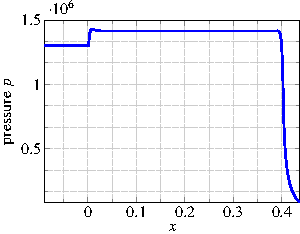
\includegraphics[width=0.45\textwidth]{./TikzFigures/thesis-figure25}
	}
	\subfloat[\label{p4.fig:5p2.2b}]{%
			\includegraphics[width=0.45\textwidth]{./TikzFigures/thesis-figure26}
	} \\
	\subfloat[\label{p4.fig:5p2.2c}]{%
			\includegraphics[width=0.45\textwidth]{./TikzFigures/thesis-figure27}
	}
	\subfloat[\label{p4.fig:5p2.2d}]{%
			\includegraphics[width=0.45\textwidth]{./TikzFigures/thesis-figure28}
	}
	\caption{\protect\subref{p4.fig:5p2.2a} Pressure profile of the steady state.  \protect\subref{p4.fig:5p2.2b} Oscillatory mode of pressure located at $x=0.36$ for the unsteady flow. \protect\subref{p4.fig:5p2.2c} Relative error between the high-fidelity and approximated pressure. \protect\subref{p4.fig:5p2.2d} Approximation of the oscillations.}
	\label{p4.fig:5p2.2}
	\end{centering}
\end{figure}

The discontinuities that appear in the solution of \eqref{p4.eq:5p2.10} suggest that a relatively large basis is required to resolve fine structures in the solution. Here, a POD basis is generated with $k=200$, $k=300$ and $k=400$ number of basis vectors. To avoid basis changes in the reduced system, only one POD basis is considered for $\rho$, $\rho u$ $\rho E$ and $\rho Y_{ox}$. The explicit SSP RK3 is then used to integrate the reduced system in time, for the unsteady system. The source terms are evaluated in the high-fidelity space and projected onto the reduced space. However, in principle, the DEIM can be applied to accelerate the evaluation of this component. 

\Cref{p4.fig:5p2.2c} shows the approximation error of the pressure, due to MOR. It is observed that the approximation is consistently improved as the number of basis vectors increases. Furthermore, the approximate solution maintains high accuracy over a relatively long time-integration. The oscillation of pressure is demonstrated in \Cref{p4.fig:5p2.2d}. The overall behaviour of pressure is well approximated by the reduced system. Similar results are obtained for a POD basis with higher number of modes.

We note that the discrete form of \eqref{p4.eq:5p2.10} is not in the full skew-symmetric form. Nonetheless, the quasi-skew-symmetric discretization offers remarkable stability preservation.

\section{Conclusions} \label{p4.sec:con}

Conservation of nonlinear invariants are not, in general, guaranteed with conventional model reduction techniques. The violation of such invariants often results in a qualitatively wrong or unstable reduced system, even when the high-fidelity system is stable. This is particularly important for fluid flow, where conservation of the energy, as a nonlinear invariant of the system, is crucial for a correct numerical evaluation.

In this paper, we discuss that conservative properties of the skew-symmetric form for fluid flow can naturally be extended to the reduced system. Conventional MOR techniques preserve the skew-symmetry of differential operator which result in the conservation of quadratic invariants at the level of the reduced system. Furthermore, the reduced system also contains quadratic invariants with respect to the reduced variables that approximates the invariants of the high-fidelity system. This results in the construction of a physically meaningful reduced system, rather than a mere couple systems of differential equations.

Numerical experiments for the incompressible and compressible Euler equation confirm conservation of mass, momentum and energy for the reduced model with the skew-symmetric discretization. In contrast, when a non-skew-symmetric form, e.g. divergence form or advective form, is considered, MOR does not necessarily yield a stable reduced system. On the other hand the skew-symmetric form consistently yields a robust reduced system over long time-integration, even when the reduced space does not represent the high-fidelity solution accurately. 

Finally, a MOR of a quasi-skew-symmetric form for the CVRC model is presented. Although this model is not in a full skew-symmetric form and an explicit Runge-Kutta method used for time-integration, we still recover a reduced model with excellent stability properties.
